\section{Introduction}
\section{Model of Computation}
\section{Related Work}
\section{Necessity of Shared Memory Garbage Collection}
\section{Contributions}

\section{Edge Classification Algorithm}
\section{Single Collector Concurrent Garbage Collection Algorithm}
\subsection{Examples}
\section{Correctness}
\begin{comment}

\documentclass{sigplanconf}
\usepackage[ruled,vlined,linesnumbered]{algorithm2e}
%
\usepackage{amssymb,amsmath,amsfonts}
\usepackage{booktabs}
\usepackage{color}
\usepackage{graphicx}
%\usepackage{subfig}
\usepackage{wrapfig}
\usepackage{verbatim}
\usepackage{enumerate}
\usepackage{hyperref,url}
%\usepackage{multicol}
\usepackage[english]{babel}
\usepackage{blindtext}
%\usepackage{float}
%\floatstyle{boxed}
%\restylefloat{figure}

\newcommand{\cO}{{\cal O}}
\newcommand{\src}{{\sc SRC}}
\newcommand{\wrc}{{\sc WRC}}

\newcommand{\todo}[1]{{\color{blue}$\blacksquare$~\textsf{[TODO: #1]}}}
\newcommand{\update}[1]{{\color{magenta}~\textsf{note:: #1}}}

\newcommand{\sq}{\hbox{\rlap{$\sqcap$}$\sqcup$}}
\newcommand{\qed}{\hspace*{\fill}\sq}
\newenvironment{proof}{\noindent {\bf Proof.}\ }{\qed\par\vskip 4mm\par}
\newenvironment{proofs}{\noindent {\bf Proof. (sketch)}\ }{\qed\par\vskip 4mm\par}
\newenvironment{corallary}{\noindent {\bf Corollary.}\ }{\qed\par\vskip 4mm\par}

\newtheorem{theorem}{Theorem}[section]
\newtheorem{lemma}[theorem]{Lemma}
\newtheorem{claim}[theorem]{Claim}
\newtheorem{fact}[theorem]{Fact}
\newtheorem{corollary}[theorem]{Corollary}
\newtheorem{definition}{Definition}
\newtheorem{observation}{Observation}
\newtheorem{invariant}{Invariant}




%\begin{comment}
\makeatletter
\def \@ivtitleauthors#1#2#3#4{%
  \if \@andp{\@emptyargp{#2}}{\@emptyargp{#3}}%
    \noindent \@setauthor{40pc}{#1}{\@false}\par
  \else\if \@emptyargp{#3}%
    \noindent \@setauthor{17pc}{#1}{\@false}\hspace{3pc}%
              \@setauthor{17pc}{#2}{\@false}\par
  \else\if \@emptyargp{#4}%
    \noindent \@setauthor{17pc}{#1}{\@false}\hspace{3pc}%
              \@setauthor{17pc}{#3}{\@false}\par
  \else
    \noindent \@setauthor{9.3333pc}{#1}{\@false}\hspace{1.5pc}%
              \@setauthor{9.3333pc}{#2}{\@false}\hspace{1.5pc}%
              \@setauthor{9.3333pc}{#3}{\@false}\hspace{1.5pc}%
              \@setauthor{9.3333pc}{#4}{\@true}\par
    \relax
  \fi\fi\fi
  \vspace{20pt}}
\def \@maketitle {%
  \begin{center}
  \@settitlebanner
  \let \thanks = \titlenote
  {\leftskip = 0pt plus 0.25\linewidth
   \rightskip = 0pt plus 0.25 \linewidth
   \parfillskip = 0pt
   \spaceskip = .7em
   \noindent \LARGE \bfseries \@titletext \par}
  \vskip 6pt
  \noindent \Large \@subtitletext \par
  \vskip 12pt
  \ifcase \@authorcount
    \@latex@error{No authors were specified for this paper}{}\or
    \@titleauthors{i}{}{}\or
    \@titleauthors{i}{ii}{}\or
    \@titleauthors{i}{ii}{iii}\or
    \@ivtitleauthors{i}{ii}{iii}{iv}\or
    \@titleauthors{i}{ii}{iii}\@titleauthors{iv}{v}{}\or
    \@titleauthors{i}{ii}{iii}\@titleauthors{iv}{v}{vi}\or
    \@titleauthors{i}{ii}{iii}\@titleauthors{iv}{v}{vi}%
                  \@titleauthors{vii}{}{}\or
    \@titleauthors{i}{ii}{iii}\@titleauthors{iv}{v}{vi}%
                  \@titleauthors{vii}{viii}{}\or
    \@titleauthors{i}{ii}{iii}\@titleauthors{iv}{v}{vi}%
                  \@titleauthors{vii}{viii}{ix}\or
    \@titleauthors{i}{ii}{iii}\@titleauthors{iv}{v}{vi}%
                  \@titleauthors{vii}{viii}{ix}\@titleauthors{x}{}{}\or
    \@titleauthors{i}{ii}{iii}\@titleauthors{iv}{v}{vi}%
                  \@titleauthors{vii}{viii}{ix}\@titleauthors{x}{xi}{}\or
    \@titleauthors{i}{ii}{iii}\@titleauthors{iv}{v}{vi}%
                  \@titleauthors{vii}{viii}{ix}\@titleauthors{x}{xi}{xii}%
  \else
    \@latex@error{Cannot handle more than 12 authors}{}%
  \fi
  \vspace{1.75pc}
  \end{center}}
\makeatother
%\end{comment}





\begin{document}

\special{papersize=8.5in,11in}
\setlength{\pdfpageheight}{\paperheight}
\setlength{\pdfpagewidth}{\paperwidth}

\conferenceinfo{ISMM~'14}{June 12 2014, Edinburgh, United Kingdom}
\copyrightyear{2014}
\copyrightdata{978-1-4503-2921-7/14/06}
%\doi{2602988.2602990}


\title{Concurrent, Parallel Garbage Collection in Linear Time}
 \authorinfo{Steven R. Brandt} {Center for Computation and Technology, School of Electrical Engineering and Computer Science, Louisiana State University, Baton Rouge, LA 70803, USA} {sbrandt@cct.lsu.edu}
 \authorinfo{Hari Krishnan} {Center for Computation and Technology, School of Electrical Engineering and Computer Science, Louisiana State University, Baton Rouge, LA 70803, USA} {hkrish4@tigers.lsu.edu}
 \authorinfo{Gokarna Sharma}{School of Electrical Engineering and Computer Science, Louisiana State University, Baton Rouge, LA 70803, USA}{gokarna@csc.lsu.edu}
 \authorinfo{Costas Busch}{School of Electrical Engineering and Computer Science,\ Louisiana State University,\ Baton Rouge, LA 70803, USA}{busch@csc.lsu.edu}

\maketitle

\sloppy
\begin{abstract}
This paper presents a new concurrent garbage collection algorithm based on two types of
reference, {\em strong} and {\em weak}, to link the graph of objects. Strong
references connect the roots to all the nodes in the graph but do not contain
cycles. Weak references may, however, contain cycles.

Advantages of this system include: (1) reduced processing, nontrivial
garbage collection work is only required when the last strong reference
is lost; (2) fewer memory traces to delete objects, a garbage cycle only needs to be traversed
twice to be deleted;
(3) fewer memory traces to retain objects, since the collector can often
prove objects are reachable without fully tracing support cycles to which the objects belong;
(4) concurrency, it can run in parallel with a live system
without ``stopping the world;'' (5) parallel, because collection operations
in different parts of the memory can proceed at the same time.

Previous variants of this technique required exponential cleanup time~\cite{Salkild1987,Pepels1988}, but
our algorithm is linear in total time, i.e. any changes in the graph
take only $\cO(N)$ time steps,
where $N$ is the number of edges in the
affected subgraph (e.g. the subgraph whose strong support is affected by the operations).
%Brownbridge's algorithm had the problem that it prematurely reclaims objects in
%some cases, and subsequent attempts due to Salkild \cite{Salkild1987} and Pepels
%et al. \cite{Pepels1988} to resolve this problem either suffered from
%non-termination or they have very high (at least exponential) clean up time. The
%Experimentation evaluation of our algorithm in Java [[]] confirm that our
%theoretical findings are in order with the practical results. \begin{comment} In
%this case we identify a subgraph of memory in which references are phantomized,
%i.e. converted to an indeterminate state that is neither weak nor strong. Once
%the phantom subgraph is complete, references are rebuilt (if possible). The
%stages of phantomizing and rebuilding are divided by a global barrier, and
%operate in a time that is linear in the number of links. It should be noted,
%however, that this barrier only applies to the operations of the garbage
%collector, and {\em not} to the running application. Apart from this barrier,
%operations within the garbage collector and the application may proceed
%concurrently without the need for ``stopping the world.''
%
%Overheads of our algorithm include a thrid reference counter type (the phantom reference) plus one bit on each object, and two
%bits on each outgoing reference.
%Our system does not use backward references of
%any kind, and can run concurrently with the application without the need for ``stopping the world.''
%\end{comment}
\end{abstract}
%{\bf Keywords}--Garbage collection; Memory management; Reference counting; Cyclic graphs; Correctness; Concurrency control
%\end{titlepage}

\category{D.3.4}{Programming Languages}{Processors--Memory management (garbage collection)}

% general terms are not compulsory anymore,
% you may leave them out
\terms
Algorithms, Performance, Experimentation, Languages, Design, Termination

\keywords
Garbage Collection,
Parallel programming theory and models,
Compilers and runtime systems,
Software for productivity parallel programming, Parallel algorithms,
Concurrent data structures
\end{comment}

\section{Introduction}
Garbage collection is an important productivity feature in many languages,
eliminating a thorny set of coding errors which can be created by explicit
memory management \cite{McBeth1963,Bacon2001,Bacon:2001:JWC,Barabash2005,Jones1996,McCarthy1960,Collins1960}. %,Wilson1992}.
%Abdullahi1998,
Despite the many advances in garbage collection, there
are problem areas which have difficulty benefiting, such as distributed
or real-time systems; see \cite{Bacon2003,Pizlo2008,Veiga2005}. %Kafura1995,
Even in more mundane settings, a certain
liveness in the cleanup of objects may be required by an application for
which the garbage collector provides little help, e.g. managing a small pool of
database connections.

The garbage collection system we propose is based on a scheme originally
proposed by Brownbridge~\cite{Brownbridge1985}. Brownbridge proposed the
use of two types of pointers: {\it strong} and {\it weak}\footnote{These references are unrelated to the weak, soft, and phantom reference objects available in Java under Reference class.}. Strong pointers
are required to connect from the {\it roots} (i.e. references from the stack or global memory) to
all nodes in the graph, and contain no cycles. A path of strong links (i.e. pointers) from the roots guarantees
that an object should be in memory. Weak pointers are available to close cycles and provide
the ability to connect nodes in arbitrary ways.




Brownbridge's proposal was
vulnerable to premature collection~\cite{Salkild1987}, and subsequent attempts
to improve it introduced poor performance
(at least exponential cleanup
time in the worst-case)~\cite{Pepels1988}; details in Section \ref{section:exponential}.
Brownbridge's core idea, however, of using two types of
reference counts was sound: maintaining this pair of reference counts allows the
system to remember a set of acyclic paths through memory so that the system can
minimize collection operations. For example, Roy et al.~\cite{Roy:1998} used Brownbridge's idea to optimize scanning in databases.
In this work we will show how the above problems with the Brownbridge collection scheme can be repaired by the inclusion of a third type of counter, which we call a {\em phantom count}. This modified system has a number of advantages.

%\update{Gokarna: The advantage of our algorithm lies on how to improve upon the performance of  Brownbridge's algorithm. The third reference phantom is used to mark all affected links. It has many benefits: (i) only }

Typical hybrid reference count and collection systems, e.g. \cite{Bacon2001,Levanoni2006,Bacon:2001:JWC,Barabash2005,Lins2008}, which use a reference counting collector combined with a tracing collector or cycle collector,
must perform nontrivial work whenever a reference count is decreased and does
not reach zero. The modified Brownbridge system, with three types of reference counts, must
perform nontrivial work only when the strong reference count reaches zero and
the weak reference count is still positive, a significant reduction \cite{Brownbridge1985,Jones1996}.

Many garbage collectors in the literature employ a generational technique, for example the generational collector proposed in \cite{Printezis:2000}, taking advantage of
the observation that younger objects are more likely to need garbage collecting
than older objects. Because the strong/weak reference system tends to make the links in long-lived paths through memory
strong, old objects connected to these paths are
unlikely to become the focus of the garbage collector's work.

In other conceptions of weak pointers, if a node is reachable by a strong pointer and a weak pointer and the strong pointer is removed, the node is garbage, and the node is deleted. In Brownbridge's conception of weak pointers, the weak pointer is turned into a strong pointer in an intelligent way.

In many situations,
the collector can update the pointer types and prove an object is still live without tracing through memory
cycles the object may participate in. For example, when root $R1$ is removed from the graph shown in Fig.~\ref{prove},
the collector
only needs to convert link 1 to strong and examine link 2 to prove that object $A$ does not need
to be collected. What's more, because the strength of the pointer depends on a combination of states in
the source and target, the transformation from strong to weak can be carried out
without the need for back-pointers (i.e. links that can be followed
from target to source as well as source to target).


This combination of effects, added to the fact that our collector can
run in parallel with a live system, may prove useful in soft real-time systems,
and may make the use of ``finalizers'' on objects more practical.
These kinds of advantages should also be significant in a distributed
setting, where traversal of links in the collector is a more expensive
operation. Moreover, when a collection operation is local, it has the opportunity to
remain local, and cleanup can proceed without any kind of global synchronization
operation.

\begin{figure}[!t]
\centering
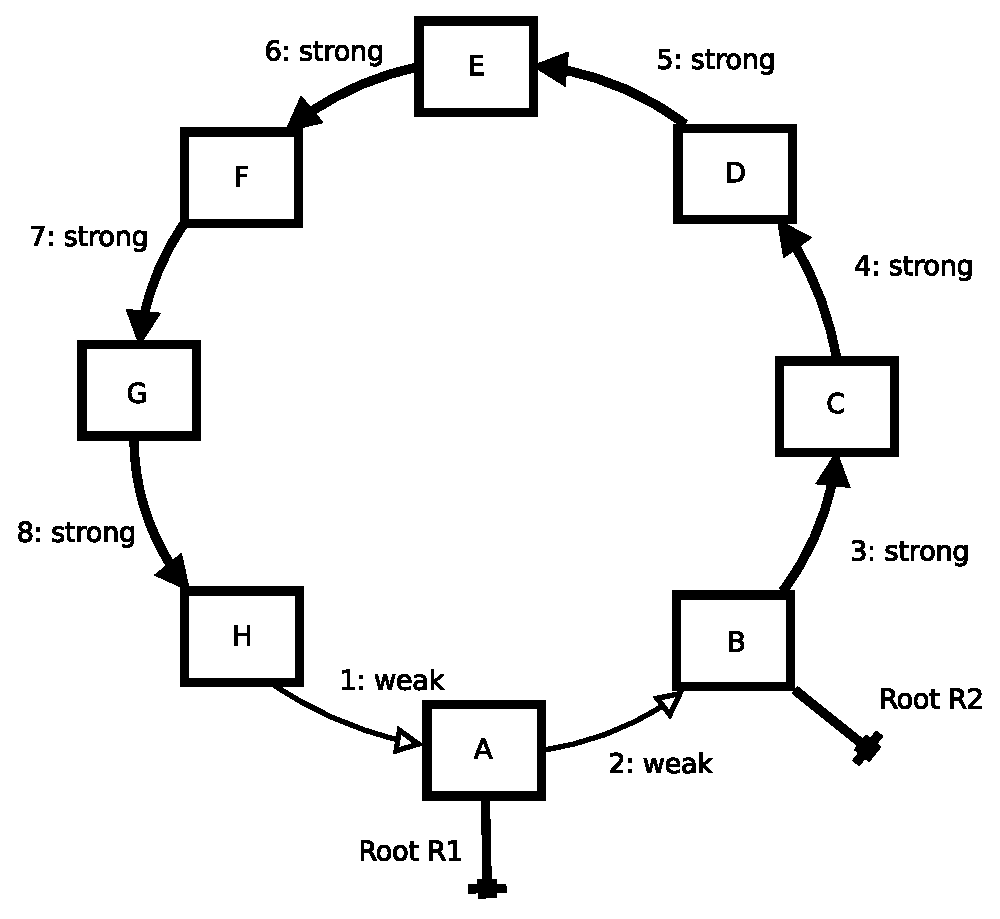
\includegraphics[width=0.32\textwidth]{figs/simplecyclenew}
\caption{When root R1 is removed, the garbage collection algorithm
only needs to trace link 2 to prove that object A does not need
to be collected.}
\label{prove}
\end{figure}

The contribution of this paper is threefold. Our algorithm never prematurely deletes any reachable object, operates in linear in time regardless of the structure (any
deletion of edges and roots takes only $\cO(N)$ time steps,
where $N$ is the number of edges in the
affected subgraph), and works concurrently with the application, without the need for system-wide pauses, i.e. ``stopping the world.''
%\update{Gokarna: We should say something like this: Moreover, our GC algorithm guarantees that no more total work is spent in the GC than in allocation (within constant factors).
%That is, a series of addition and deletion of edges do not increase the cost of collection dramatically.
%First we need to figure what Baker proved back in 1978. either outline guarantees similar to Baker or say it does not apply }
This is in contrast to Brownbridge's original algorithm and its variants \cite{Brownbridge1985,Salkild1987,Pepels1988} which can not handle concurrency issues that arise in modern multiprocessor architectures~\cite{Roy:1998}.

Our algorithm does, however, add a third kind of pointer, a {\em phantom pointer}, which identifies a temporary state that is neither strong nor weak. The addition of the space overhead offsets the time overhead in Brownbridge's work.

%Our contribution does not consist of a production-ready nor a fully optimized collector.
%Rather, we provide a proof-of-concept implementation that emphasizes correctness and time complexity.% The
%use of strong/weak pointer types provides an avenue for reduced reference traversal which
%should be especially beneficial in a distributed setting.


\subsection{Most Related Work: Premature Collection, Non-termination, and Exponential Cleanup Time}
\label{section:exponential}
Before giving details of our algorithm in Section \ref{section:high-level} %and giving details in Section \ref{section:algorithm}
-- which in turn is a modification of Brownbridge's algorithm and its variants \cite{Brownbridge1985,Salkild1987,Pepels1988} -- we first describe the problems with previous variants. In doing so, we follow the description given in the excellent garbage collection book due to Jones and Lins \cite{Jones1996}.

It was proven by McBeth \cite{McBeth1963} in early sixties that reference counting collectors were unable to handle cyclic structures; several attempts to fix this problem appeared subsequently, e.g. \cite{Friedman1979,Bobrow1980,Lins2008}. We give details in Section \ref{subsection:otherrelated}.
In contrast to the approach followed in \cite{Friedman1979,Bobrow1980,Lins2008} and several others,
Brownbridge \cite{Brownbridge1985} proposed, in 1985, a strong/weak pointer algorithm to tackle the problem of reclaiming cyclic data structures by distinguishing cycle closing pointers (weak pointers) from other references (strong pointers) \cite{Jones1996}. %different algorithm to tackle the problem of reclaiming cyclic structures using strong and weak pointers.
This algorithm relied on maintaining two invariants: (a) there are no cycles in strong pointers and (b) all items in the graph must be strongly reachable from the roots.

Some years after the publication, Salkild \cite{Salkild1987} showed that Brownbridge's algorithm
\cite{Brownbridge1985} could reclaim objects prematurely in some
configurations, e.g. a double cycle. If the last strong pointer (or link) to
an object in one cycle but not the other was lost, Brownbridge's
method would incorrectly claim nodes from the cycle.
Salkild \cite{Salkild1987} corrected this problem by proposing
that if the last strong link was removed from an object which still
had weak pointers, a collection process should re-start from that node.
While this approach eliminated the premature deletion problem, it introduced a
potential non-termination problem.

Subsequently, Pepels et al.~\cite{Pepels1988} proposed a new algorithm based on
Brownbridge-Salkild's algorithm and solved the problem of non-termination by
using a marking scheme. In their algorithm, they used two kinds of mark: one to
prevent an infinite number of searches, and the other to guarantee termination
of each search. Although correct and terminating, Pepels et al.'s algorithm is far more
complex than Brownbridge-Salkild's algorithm and in some cyclic structures the
cleanup cost complexity becomes at least
exponential in the worst-case \cite{Jones1996}. This is due to the fact that when
cycles occur, whole state space searches from
each node in the cyclic graph must be initiated, possibly many times. After Pepels et al.'s algorithm, we are not aware
of any other work on reducing the cleanup cost or complexity of the Brownbridge
algorithm. Moreover, there is no concurrent collection technique using this approach which can be applicable for the garbage collection in modern multiprocessors.

The algorithm we present in this paper removes all the limitations described above.
Our algorithm does not perform searches as such.
Instead, whenever a node
loses its last strong reference and still has weak references, it marks all
affected links as phantom. When this process is complete for
a subgraph, the system recovers the affected subgraph by converting phantom
links to either strong or weak. Because this process is a transformation from
weak or strong to phantom, and from phantom to weak or strong, it has at most
two steps and is, therefore, manifestly linear in the number of links, i.e. it
has a complexity of only $\cO(N)$ time steps,
where $N$ is the number of edges in the
affected subgraph. Moreover, in contrast to Brownbridge's algorithm, our algorithm is concurrent and is suitable for multiprocessors.

\subsection{Other Related Work}
\label{subsection:otherrelated}
Garbage collection is
an automatic memory management technique which is considered to be an important tool for developing fast as well as reliable software.  Garbage collection has been studied extensively in computer science for more than five decades, e.g., \cite{McBeth1963,Brownbridge1985,Salkild1987,Pepels1988,Bacon2001,Bacon:2001:JWC,Barabash2005,Jones1996}. %,Wilson1992}. %We refer readers to these books \cite{Jones1996,Jones2011} and these surveys \cite{Chase1987,Wilson1992} for the overview of the research in this field.
Reference counting is a widely-used form of garbage collection whereby each object has a count of the number of references to it; garbage is identified by having a reference count of zero \cite{Bacon2001}.
Reference counting approaches were first developed for LISP by Collins \cite{Collins1960}.
% in the context of a process suspension problem in LISP \cite{McCarthy1960}.
%Improvements to the initial algorithms were proposed in several subsequent papers.
Improved variations were proposed in several subsequent papers, e.g. \cite{Friedman1979,Hughes1987,Jones1996,Lins2008,Levanoni2006}. We direct readers to Shahriyar et al.~\cite{Shahriyar:2012} for the valuable overview of the current state of reference counting collectors.

It was noticed by McBeth \cite{McBeth1963} in early sixties that reference counting collectors were unable to handle cyclic structures.
After that several reference counting collectors were developed, e.g. \cite{Friedman1979,Bobrow1980,Lins:1992:CRC,Lins:2002:EAC}.
The algorithm in Friedman \cite{Friedman1979} dealt with recovering cyclic data in immutable structures, whereas Bobrow's algorithm \cite{Bobrow1980}
can reclaim all cyclic structures but relies on the explicit
information provided by the programmer. 
Trial deletion approach was studied by Christopher \cite{Christopher1984} which tries to collect cycles by identifying groups of self-sustaining objects. 
Lins \cite{Lins:1992:CRC} used a cyclic buffer to reduce repeated scanning of the same nodes in their mark-scan algorithm for cyclic reference counting. Moreover, in \cite{Lins:2002:EAC}, Lins improved his algorithm  from \cite{Lins:1992:CRC} by eliminating the scan operation through the use of a Jump-stack data structure.
%Reference counting garbage collectors developed recently were augmented with either a tracing collector or a cycle detector to reclaim cyclic structures, e.g. \cite{Bacon2001,Paz2007,Lins2008}.
%We refer the reader to \cite{Abdullahi1998,Jones2011} for details.
%For example, the reference counting collector proposed in \cite{Paz2007} combines the sliding view collector of \cite{Levanoni2006} with the cycle collector of \cite{Bacon2001}.


%Friedman and Wise's algorithm \cite{Friedman1979} was specialized to recovering cyclic data in immutable structures. Bobrow's algorithm \cite{Bobrow1980}
%can reclaim all cyclic structures but relies on the explicit
%information provided by the programmer. Hughes\cite{Hughes1987}, in his unpublished note, improved Bobrow's algorithm by avoiding the need of the extra information provided by the programmer.
%The details of other subsequent work is this area can be found in \cite{Chase1987,Wilson1992,Jones1996,Jones2011,Lins2006,Lins2008,Levanoni2006,Axford1990}.

% and some recent work on cyclic reference counting is in \cite{Lins2006,Lins2008,,Levanoni2006}.

%In 1985, Brownbridge \cite{Brownbridge1985} proposed a different algorithm to tackle the problem of reclaiming cyclic structures using strong and weak pointers. This algorithm was relied on maintaining two invariants: (a) there are no cycles in strong pointers and (b) all items in the graph must be strongly reachable from the root node. Unfortunately, his algorithm was shown incorrect by  Salkild \cite{Salkild1987}. Salkild observed that Brownbridge's algorithm sometimes reclaims objects prematurely and gave a new algorithm that corrected Brownbridge's algorithm in \cite{Salkild1987}. However, this algorithm suffers from non-termination in certain situations due to the fact that it may need infinite number of searches to determine the garbage cells. Pepels et al.~\cite{Pepels1988} proposed a new algorithm based on Brownbridge-Salkild's
%algorithm and solved the problem of non-termination by using a marking scheme. In their algorithm, they used two kinds of mark: one to prevent an infinite number of searches, and the other to guarantee termination of each search. Although correct and terminating, the algorithm is far more complex than  Brownbridge-Salkild's algorithm and in some cyclic structures the cleanup cost complexity of Pepel et al.'s algorithm becomes exponential in the worst-case \cite{Jones1996}.
%After Pepel et al.'s algorithm, we are not aware of any other work on making the cleanup cost complexity of Brownbridge's algorithm linear.
%The algorithm we present in this paper removes all the limitations of original Brownbridge's algorithm \cite{Brownbridge1985} and also its variants \cite{Salkild1987,Pepels1988} and provides linear number of searches, guarantees termination, and limits the cleanup cost complexity to $\cO(N)$, in the worst-case, where $N$ is the number of cells in a cycle.

%mark-sweep \cite{Cohen1967}.

%\input{distributed_refs}

% Note: Gokarna had a lot of this backwards. He was contrasting reference counting
% to stop-the-world collectors, and the kinds of write barriers he was concerned with
% are present in our system.
With the advancement of multiprocessor architectures,
reference counting garbage collectors have become popular because
they do not require all application threads to be stopped before the garbage collection algorithm can run~\cite{Levanoni2006}.
Recent work in reference counting algorithms, e.g. \cite{Barabash2005,Levanoni2006,Bacon2001,Bacon:2001:JWC}, try to
reduce concurrent operations and increase the efficiency of reference counting collectors.
Since our collector is a reference counting collector, it can potentially benefit from the
same types of optimizations discussed here. We leave that, however, to a future work.

%In contrast to simple stop-the-world garbage collectors which completely halt execution of the application to run a collection cycle, concurrent garbage collectors (and also incremental garbage collectors, e.g. \cite{Barabash2005}) interleave the collection cycles with the application to reduce the
%disruption of the stop-the-world approach.
%However, reference counting based garbage collectors have an inherence limitation with respect to concurrency in multiprocessor architectures in the sense that the update of the reference
%counts must be atomic since they are being updated by all
%application threads, and, when updating a pointer,
%a thread must know the previous value of the pointer-slot
%being updated despite many parallel writes from concurrent application threads \cite{Levanoni2006}.
%
%remove the requirement of atomic and synchronization operations for updating pointers and reference counts while running them on multiprocessors and also
%
%% Therefore,
%in order to make better use of the processing capacity and the parallelism  available in multiprocessors, reference counting based concurrent
%collectors have been presented and studied, e.g. \cite{Barabash2005,Levanoni2006,Bacon2001,Bacon:2001:JWC}. % garbage collection is also considered for several other particular systems, namely concurrent systems, real-time systems, mobile actor systems, and asynchronous distributed systems \cite{Pizlo2008,Huelsbergen1998,Wang2006,Wang2010,Kafura1995,Veiga2005}. Pizlo et al. \cite{Pizlo2008} studied concurrent real-time garbage collectors.
%However, reference counting based garbage collectors have an inherence limitation with respect to concurrency in multiprocessor architectures in the sense that the update of the reference
%counts must be atomic since they are being updated by all
%application threads, and, when updating a pointer,
%a thread must know the previous value of the pointer-slot
%being updated despite many parallel writes from concurrent application threads \cite{Levanoni2006}.
%Therefore, these papers \cite{Barabash2005,Levanoni2006,Bacon2001,Bacon:2001:JWC} shed light on how to obtain better algorithms by focusing thoroughly on reducing synchronization requirements and improving throughput and latency.

However, as mentioned earlier, reference counting garbage collectors cannot collect cycles \cite{McBeth1963}. Therefore, concurrent reference counting collectors \cite{Barabash2005,Levanoni2006,Bacon2001,Bacon:2001:JWC,Paz2007,Lins2008} use other techniques, e.g. they supplement the reference counter with a tracing collector or a cycle detector, together with their concurrent reference counting algorithm. For example, the reference counting collector proposed in \cite{Paz2007} combines the sliding view reference counting concurrent collector of \cite{Levanoni2006} with the cycle collector of \cite{Bacon2001}. Our collector has some similarity with these, in that our $Phantomization$ process may traverse many nodes. It should, however, trace fewer nodes and do so less frequently. Recently, Frampton provides a detailed study of cycle collection in his PhD thesis \cite{Frampton2010}.
%To the best of our knowledge, we are not aware of any existing reference counting algorithm that itself can reclaim cycles.
%\todo{Steve: is it OK to say this statement}
%We note here that it is challenging to develop a variation of referencing counting collectors which collect cycles without the need of an auxiliary collector dedicated for reclaiming cycles. Our algorithm is a significant step towards this direction. xxx

%a backup tracing collector or a cycle detector to reclaim cyclic structures \cite{Bacon2001,Paz2007,Lins2008}.

%Otherwise, a confusion occurs in the bookkeeping of
%the reference counts. Thus, the naive solution requires a lock
%on any update operation. More advanced solutions have recently reduced this overhead to a compare-and-swap operation, which is still a time consuming write-barrier. Recent developments lead to better algorithm \cite{Levanoni2006}\cite{Barabash2005} based on reference counting but they can not collect cycles. They used mark-and-sweep algorithm together with the reference counting algorithm \cite{Levanoni2006}.
%Bacon et al. \cite{Bacon2001,Bacon:2001:JWC} also studied on-the-fly reference counting algorithms for multiprocessors. These all work focused on reducing synchronization and improving throughput and latency. They did not elaborate further on how to avoid the limitations of reference counting algorithms in reclaiming cycles.
%Huelsbergen and Winterbottom \cite{Huelsbergen1998} extended the mark-and-sweep garbage collection technique to a concurrent setting.
%A parallel, incremental, mostly concurrent garbage collector for servers is given in \cite{Barabash2005}.

%Recently, garbage collection is also considered for several other particular systems, namely concurrent systems, real-time systems, mobile actor systems, and asynchronous distributed systems \cite{Pizlo2008,Huelsbergen1998,Wang2006,Wang2010,Kafura1995,Veiga2005}. Pizlo et al. \cite{Pizlo2008} studied concurrent real-time garbage collectors.
%Huelsbergen and Winterbottom \cite{Huelsbergen1998} extended the mark-and-sweep garbage collection technique to a concurrent setting.
%A parallel, incremental, mostly concurrent garbage collector for servers is given in \cite{Barabash2005}.
%%Distributed garbage collection for mobile actor systems is studied in several papers, e.g. \cite{Wang2006,Wang2010}, using the pseudo root approach and also through vertex-preserving actor-to-object graph transformations.
%%Veiga and Ferreira \cite{Veiga2005} presented a garbage collection technique for asynchronous distributed systems.
%%Kafura et al. \cite{Kafura1995} presented a distributed and concurrent garbage collection algorithm for active objects. Their algorithm is snapshot based.



Herein we have tried to cover a sampling of garbage collectors that are most relevant to our work.

Apple's ARC memory management system makes a distinction between ``strong'' and ``weak'' pointers, similar to what we describe here. In the ARC memory system, however, the type of each pointer must be specifically designated by the programmer, and this type will not change during the program's execution. If the programmer gets the type wrong, it is possible for ARC to have strong cycles as well as prematurely deleted objects. With our system, the pointer type is automatic and can change during the execution. Our system protects against these possibilities, at the cost of lower efficiency.

There exist other concurrent techniques optimized for both uniprocessors as well as multiprocessors. Generational concurrent garbage collectors were also studied, e.g. \cite{Printezis:2000}. Huelsbergen and Winterbottom \cite{Huelsbergen1998} proposed an incremental algorithm for the concurrent garbage collection that is a variant of mark-and-sweep collection scheme first proposed in \cite{McCarthy1960}.
%Recently, McGachey et al. \cite{McGachey2008} considered how to build a concurrent garbage collector from a state of the art software transactional memory system \cite{Shavit1997}. 
Furthermore, garbage collection is also considered for several other systems, namely real-time systems %, mobile actor systems, 
and asynchronous distributed systems, e.g. \cite{Pizlo2008,Veiga2005}. %Wang2010,Huelsbergen1998,Kafura1995,
%However, we do not explore this area in this present work, but we conjecture that our technique can be useful to these systems and deserves further work (some possible directions are outlined in Section \ref{section:future-work}).

%Brownbridge's algorithm \cite{Brownbridge1985}, and its subsequent improvements due to Salkild\cite{Salkild1987}, and Pepels et al. \cite{Pepels1988}, which we describe later in Section \ref{section:exponential}.

Concurrent collectors are gaining popularity. The concurrent collector described in Bacon and Rajan~\cite{Bacon2001} can be considered to be one of the more efficient reference counting concurrent collectors. The algorithm uses two counters per object, one for the actual reference count and other for the cyclic reference count. Apart from the number of the counters used, the cycle detection strategy requires a minimum of two traversals of cycle when the cycle is reachable and eleven cycle traversals when the cycle is garbage.
%The necessity of eleven traversals of cyclic objects for safety conditions and difficulty in making the algorithm parallel easily began as the motivation of the work. So our work concentrates on the concurrency as well as parallel aspect of the collectors along with amortizing the number of the traversal required in the cycle detection strategies. Our approach uses two traversals for the deletion of the cycle and needs two traversal of the affected graph when the object is speculated wrongly as cycle. So we give tight upper bound on the number of the traversal happens in the affected graph for every event in the graph.

%\todo{Hari, say something more about \cite{Bacon2003,Bacon2001,Bacon:2001:JWC}}


\subsection{Paper Organization}
The rest of the paper is organized as follows. We present %the high level overview of
our strong/weak/phantom pointer based concurrent garbage collector in Section~\ref{section:high-level} with some examples. %We then give the details of the collector in Section~\ref{section:algorithm}.
In Section~\ref{section:correctness}, we sketch proofs of its correctness and complexity properties. In Section~\ref{section:experimental}, we give some experimental results. We conclude the paper with future research directions in Section~\ref{section:future-work} and a short discussion in Section~\ref{section:conclusion}. Detailed algorithms may be found in the appendix.
% The source code of our concurrent collector implementation can be found in~\cite{url:refimpl}.

%\subsection{Other Related Work}
\label{subsection:otherrelated}
Garbage collection is
an automatic memory management technique which is considered to be an important tool for developing fast as well as reliable software.  Garbage collection has been studied extensively in computer science for more than five decades, e.g., \cite{McBeth1963,Brownbridge1985,Salkild1987,Pepels1988,Bacon2001,Bacon:2001:JWC,Barabash2005,Jones1996}. %,Wilson1992}. %We refer readers to these books \cite{Jones1996,Jones2011} and these surveys \cite{Chase1987,Wilson1992} for the overview of the research in this field.
Reference counting is a widely-used form of garbage collection whereby each object has a count of the number of references to it; garbage is identified by having a reference count of zero \cite{Bacon2001}.
Reference counting approaches were first developed for LISP by Collins \cite{Collins1960}.
% in the context of a process suspension problem in LISP \cite{McCarthy1960}.
%Improvements to the initial algorithms were proposed in several subsequent papers.
Improved variations were proposed in several subsequent papers, e.g. \cite{Friedman1979,Hughes1987,Jones1996,Lins2008,Levanoni2006}. We direct readers to Shahriyar et al.~\cite{Shahriyar:2012} for the valuable overview of the current state of reference counting collectors.

It was noticed by McBeth \cite{McBeth1963} in early sixties that reference counting collectors were unable to handle cyclic structures.
After that several reference counting collectors were developed, e.g. \cite{Friedman1979,Bobrow1980,Lins:1992:CRC,Lins:2002:EAC}.
The algorithm in Friedman \cite{Friedman1979} dealt with recovering cyclic data in immutable structures, whereas Bobrow's algorithm \cite{Bobrow1980}
can reclaim all cyclic structures but relies on the explicit
information provided by the programmer. 
Trial deletion approach was studied by Christopher \cite{Christopher1984} which tries to collect cycles by identifying groups of self-sustaining objects. 
Lins \cite{Lins:1992:CRC} used a cyclic buffer to reduce repeated scanning of the same nodes in their mark-scan algorithm for cyclic reference counting. Moreover, in \cite{Lins:2002:EAC}, Lins improved his algorithm  from \cite{Lins:1992:CRC} by eliminating the scan operation through the use of a Jump-stack data structure.
%Reference counting garbage collectors developed recently were augmented with either a tracing collector or a cycle detector to reclaim cyclic structures, e.g. \cite{Bacon2001,Paz2007,Lins2008}.
%We refer the reader to \cite{Abdullahi1998,Jones2011} for details.
%For example, the reference counting collector proposed in \cite{Paz2007} combines the sliding view collector of \cite{Levanoni2006} with the cycle collector of \cite{Bacon2001}.


%Friedman and Wise's algorithm \cite{Friedman1979} was specialized to recovering cyclic data in immutable structures. Bobrow's algorithm \cite{Bobrow1980}
%can reclaim all cyclic structures but relies on the explicit
%information provided by the programmer. Hughes\cite{Hughes1987}, in his unpublished note, improved Bobrow's algorithm by avoiding the need of the extra information provided by the programmer.
%The details of other subsequent work is this area can be found in \cite{Chase1987,Wilson1992,Jones1996,Jones2011,Lins2006,Lins2008,Levanoni2006,Axford1990}.

% and some recent work on cyclic reference counting is in \cite{Lins2006,Lins2008,,Levanoni2006}.

%In 1985, Brownbridge \cite{Brownbridge1985} proposed a different algorithm to tackle the problem of reclaiming cyclic structures using strong and weak pointers. This algorithm was relied on maintaining two invariants: (a) there are no cycles in strong pointers and (b) all items in the graph must be strongly reachable from the root node. Unfortunately, his algorithm was shown incorrect by  Salkild \cite{Salkild1987}. Salkild observed that Brownbridge's algorithm sometimes reclaims objects prematurely and gave a new algorithm that corrected Brownbridge's algorithm in \cite{Salkild1987}. However, this algorithm suffers from non-termination in certain situations due to the fact that it may need infinite number of searches to determine the garbage cells. Pepels et al.~\cite{Pepels1988} proposed a new algorithm based on Brownbridge-Salkild's
%algorithm and solved the problem of non-termination by using a marking scheme. In their algorithm, they used two kinds of mark: one to prevent an infinite number of searches, and the other to guarantee termination of each search. Although correct and terminating, the algorithm is far more complex than  Brownbridge-Salkild's algorithm and in some cyclic structures the cleanup cost complexity of Pepel et al.'s algorithm becomes exponential in the worst-case \cite{Jones1996}.
%After Pepel et al.'s algorithm, we are not aware of any other work on making the cleanup cost complexity of Brownbridge's algorithm linear.
%The algorithm we present in this paper removes all the limitations of original Brownbridge's algorithm \cite{Brownbridge1985} and also its variants \cite{Salkild1987,Pepels1988} and provides linear number of searches, guarantees termination, and limits the cleanup cost complexity to $\cO(N)$, in the worst-case, where $N$ is the number of cells in a cycle.

%mark-sweep \cite{Cohen1967}.

%\input{distributed_refs}

% Note: Gokarna had a lot of this backwards. He was contrasting reference counting
% to stop-the-world collectors, and the kinds of write barriers he was concerned with
% are present in our system.
With the advancement of multiprocessor architectures,
reference counting garbage collectors have become popular because
they do not require all application threads to be stopped before the garbage collection algorithm can run~\cite{Levanoni2006}.
Recent work in reference counting algorithms, e.g. \cite{Barabash2005,Levanoni2006,Bacon2001,Bacon:2001:JWC}, try to
reduce concurrent operations and increase the efficiency of reference counting collectors.
Since our collector is a reference counting collector, it can potentially benefit from the
same types of optimizations discussed here. We leave that, however, to a future work.

%In contrast to simple stop-the-world garbage collectors which completely halt execution of the application to run a collection cycle, concurrent garbage collectors (and also incremental garbage collectors, e.g. \cite{Barabash2005}) interleave the collection cycles with the application to reduce the
%disruption of the stop-the-world approach.
%However, reference counting based garbage collectors have an inherence limitation with respect to concurrency in multiprocessor architectures in the sense that the update of the reference
%counts must be atomic since they are being updated by all
%application threads, and, when updating a pointer,
%a thread must know the previous value of the pointer-slot
%being updated despite many parallel writes from concurrent application threads \cite{Levanoni2006}.
%
%remove the requirement of atomic and synchronization operations for updating pointers and reference counts while running them on multiprocessors and also
%
%% Therefore,
%in order to make better use of the processing capacity and the parallelism  available in multiprocessors, reference counting based concurrent
%collectors have been presented and studied, e.g. \cite{Barabash2005,Levanoni2006,Bacon2001,Bacon:2001:JWC}. % garbage collection is also considered for several other particular systems, namely concurrent systems, real-time systems, mobile actor systems, and asynchronous distributed systems \cite{Pizlo2008,Huelsbergen1998,Wang2006,Wang2010,Kafura1995,Veiga2005}. Pizlo et al. \cite{Pizlo2008} studied concurrent real-time garbage collectors.
%However, reference counting based garbage collectors have an inherence limitation with respect to concurrency in multiprocessor architectures in the sense that the update of the reference
%counts must be atomic since they are being updated by all
%application threads, and, when updating a pointer,
%a thread must know the previous value of the pointer-slot
%being updated despite many parallel writes from concurrent application threads \cite{Levanoni2006}.
%Therefore, these papers \cite{Barabash2005,Levanoni2006,Bacon2001,Bacon:2001:JWC} shed light on how to obtain better algorithms by focusing thoroughly on reducing synchronization requirements and improving throughput and latency.

However, as mentioned earlier, reference counting garbage collectors cannot collect cycles \cite{McBeth1963}. Therefore, concurrent reference counting collectors \cite{Barabash2005,Levanoni2006,Bacon2001,Bacon:2001:JWC,Paz2007,Lins2008} use other techniques, e.g. they supplement the reference counter with a tracing collector or a cycle detector, together with their concurrent reference counting algorithm. For example, the reference counting collector proposed in \cite{Paz2007} combines the sliding view reference counting concurrent collector of \cite{Levanoni2006} with the cycle collector of \cite{Bacon2001}. Our collector has some similarity with these, in that our $Phantomization$ process may traverse many nodes. It should, however, trace fewer nodes and do so less frequently. Recently, Frampton provides a detailed study of cycle collection in his PhD thesis \cite{Frampton2010}.
%To the best of our knowledge, we are not aware of any existing reference counting algorithm that itself can reclaim cycles.
%\todo{Steve: is it OK to say this statement}
%We note here that it is challenging to develop a variation of referencing counting collectors which collect cycles without the need of an auxiliary collector dedicated for reclaiming cycles. Our algorithm is a significant step towards this direction. xxx

%a backup tracing collector or a cycle detector to reclaim cyclic structures \cite{Bacon2001,Paz2007,Lins2008}.

%Otherwise, a confusion occurs in the bookkeeping of
%the reference counts. Thus, the naive solution requires a lock
%on any update operation. More advanced solutions have recently reduced this overhead to a compare-and-swap operation, which is still a time consuming write-barrier. Recent developments lead to better algorithm \cite{Levanoni2006}\cite{Barabash2005} based on reference counting but they can not collect cycles. They used mark-and-sweep algorithm together with the reference counting algorithm \cite{Levanoni2006}.
%Bacon et al. \cite{Bacon2001,Bacon:2001:JWC} also studied on-the-fly reference counting algorithms for multiprocessors. These all work focused on reducing synchronization and improving throughput and latency. They did not elaborate further on how to avoid the limitations of reference counting algorithms in reclaiming cycles.
%Huelsbergen and Winterbottom \cite{Huelsbergen1998} extended the mark-and-sweep garbage collection technique to a concurrent setting.
%A parallel, incremental, mostly concurrent garbage collector for servers is given in \cite{Barabash2005}.

%Recently, garbage collection is also considered for several other particular systems, namely concurrent systems, real-time systems, mobile actor systems, and asynchronous distributed systems \cite{Pizlo2008,Huelsbergen1998,Wang2006,Wang2010,Kafura1995,Veiga2005}. Pizlo et al. \cite{Pizlo2008} studied concurrent real-time garbage collectors.
%Huelsbergen and Winterbottom \cite{Huelsbergen1998} extended the mark-and-sweep garbage collection technique to a concurrent setting.
%A parallel, incremental, mostly concurrent garbage collector for servers is given in \cite{Barabash2005}.
%%Distributed garbage collection for mobile actor systems is studied in several papers, e.g. \cite{Wang2006,Wang2010}, using the pseudo root approach and also through vertex-preserving actor-to-object graph transformations.
%%Veiga and Ferreira \cite{Veiga2005} presented a garbage collection technique for asynchronous distributed systems.
%%Kafura et al. \cite{Kafura1995} presented a distributed and concurrent garbage collection algorithm for active objects. Their algorithm is snapshot based.



Herein we have tried to cover a sampling of garbage collectors that are most relevant to our work.

Apple's ARC memory management system makes a distinction between ``strong'' and ``weak'' pointers, similar to what we describe here. In the ARC memory system, however, the type of each pointer must be specifically designated by the programmer, and this type will not change during the program's execution. If the programmer gets the type wrong, it is possible for ARC to have strong cycles as well as prematurely deleted objects. With our system, the pointer type is automatic and can change during the execution. Our system protects against these possibilities, at the cost of lower efficiency.

There exist other concurrent techniques optimized for both uniprocessors as well as multiprocessors. Generational concurrent garbage collectors were also studied, e.g. \cite{Printezis:2000}. Huelsbergen and Winterbottom \cite{Huelsbergen1998} proposed an incremental algorithm for the concurrent garbage collection that is a variant of mark-and-sweep collection scheme first proposed in \cite{McCarthy1960}.
%Recently, McGachey et al. \cite{McGachey2008} considered how to build a concurrent garbage collector from a state of the art software transactional memory system \cite{Shavit1997}. 
Furthermore, garbage collection is also considered for several other systems, namely real-time systems %, mobile actor systems, 
and asynchronous distributed systems, e.g. \cite{Pizlo2008,Veiga2005}. %Wang2010,Huelsbergen1998,Kafura1995,
%However, we do not explore this area in this present work, but we conjecture that our technique can be useful to these systems and deserves further work (some possible directions are outlined in Section \ref{section:future-work}).

%Brownbridge's algorithm \cite{Brownbridge1985}, and its subsequent improvements due to Salkild\cite{Salkild1987}, and Pepels et al. \cite{Pepels1988}, which we describe later in Section \ref{section:exponential}.

Concurrent collectors are gaining popularity. The concurrent collector described in Bacon and Rajan~\cite{Bacon2001} can be considered to be one of the more efficient reference counting concurrent collectors. The algorithm uses two counters per object, one for the actual reference count and other for the cyclic reference count. Apart from the number of the counters used, the cycle detection strategy requires a minimum of two traversals of cycle when the cycle is reachable and eleven cycle traversals when the cycle is garbage.
%The necessity of eleven traversals of cyclic objects for safety conditions and difficulty in making the algorithm parallel easily began as the motivation of the work. So our work concentrates on the concurrency as well as parallel aspect of the collectors along with amortizing the number of the traversal required in the cycle detection strategies. Our approach uses two traversals for the deletion of the cycle and needs two traversal of the affected graph when the object is speculated wrongly as cycle. So we give tight upper bound on the number of the traversal happens in the affected graph for every event in the graph.

%\todo{Hari, say something more about \cite{Bacon2003,Bacon2001,Bacon:2001:JWC}}

%
%\section{Previous Approaches: Non-termination and Exponential Cleanup Time}
%\label{section:exponential}
%Before introducing our algorithm -- which in turn is a modification of Brownbridge's algorithm and its variants \cite{Brownbridge1985,Salkild1987,Pepels1988} -- we first describe the Brownbridge variants and the problems of these approaches. We follow the description given in the excellent garbage collection book due to Jones and Lins \cite{Jones1996}.
%
%In 1985, Brownbridge \cite{Brownbridge1985} proposed a weak-pointer algorithm to tackle the problem of reclaiming cyclic data structures by distinguishing cycle closing pointers (weak pointers) from other references (strong pointers) \cite{Jones1996}. %different algorithm to tackle the problem of reclaiming cyclic structures using strong and weak pointers.
%This algorithm relied on maintaining two invariants: (a) there are no cycles in strong pointers and (b) all items in the graph must be strongly reachable from the root node.
%
%Salkild \cite{Salkild1987} showed that Brownbridge's algorithm
%\cite{Brownbridge1985} could reclaim objects prematurely in some
%configurations, e.g. a double cycle. If the last strong link to
%an object in one cycle but not the other was lost, Brownbridge's
%method would incorrectly claim nodes from the cycle.
%
%Salkild \cite{Salkild1987} corrected this problem by proposing
%that if the last strong link was removed from an object which still
%had weak pointers, a collection process should re-start from that node.
%While this eliminated the premature deletion problem, it introduced a
%potential non-termination problem.
%
%Pepels et al.~\cite{Pepels1988} proposed a new algorithm based on
%Brownbridge-Salkild's algorithm and solved the problem of non-termination by
%using a marking scheme. In their algorithm, they used two kinds of mark: one to
%prevent an infinite number of searches, and the other to guarantee termination
%of each search. Although correct and terminating, the algorithm is far more
%complex than Brownbridge-Salkild's algorithm and in some cyclic structures the
%cleanup cost complexity of Pepels et al.'s algorithm becomes at least
%exponential in the worst-case \cite{Jones1996}. This is due to the fact that in
%cyclic situations, this algorithm needs to perform whole state space search from
%each node in the cyclic graph. After Pepels et al.'s algorithm, we are not aware
%of any other work on reducing the cleanup cost or complexity of the Brownbridge
%algorithm.
%
%The algorithm we present in this paper removes all the limitations described
%above. Our algorithm does not perform searches, as such. Instead, whenever a node
%loses its last strong reference and still has weak references, it marks all
%affected links as phantom. When this process is complete for
%a subgraph, the system recovers the affected subgraph by converting phantom
%links to either strong or weak. Because this process is a transformation from
%weak or strong to phantom, and from phantom to weak or strong, it has at most
%two steps and is, therefore, manifestly linear in the number of links, i.e. it
%has a complexity of $\cO(N)$, where $N$ is the number of links in a subgraph.

\section{Algorithm}
\label{section:high-level}
In this section, we present our concurrent garbage collection algorithm.
%The pseudocode description of our collector is given in Algorithms \ref{algorithm:linkset}--\ref{algorithm:cleanup}.
Each object in the heap contains three reference counts: the first
two are the strong and weak, the third is the phantom count. Each object also
contains a bit named {\tt which} (Brownbridge \cite{Brownbridge1985} called it the ``strength-bit'')
to identify which of the first two counters is
used to keep track of strong references, as well as a boolean called {\tt
phantomized} to keep track of whether the node is phantomized.
Outgoing links (i.e., pointers) to other objects must also contain (1) a {\tt which} bit to
identify which reference counter on the target object they increment, and (2) a {\tt
phantom} boolean to identify whether they have been phantomized. This data structure for each object can be seen in the example given in Fig.~\ref{ex1}.

%Local creation of links only allows the creation of strong references when no
%cycle creation is possible. This includes links from (i) all root
%references i.e. references from the stack or global space; (ii) all links made from
%objects who have no strong links from other objects, i.e. objects whose only strong
%links are from roots; (iii) all links made to objects with no
%outgoing links, i.e. right after object creation and before outgoing references are
%initialized; and (iv) all objects whose outgoing links are phantomized. All
%self-references are weak. Any other link is created weak. See Algorithm~\ref{algorithm:linkset}.

Local creation of links only allows the creation of strong references when no
cycle creation is possible. Consider the creation of a link from a source object $S$
to a target object $T$. The link will be created strong if (i) the only strong
links to $S$ are from roots i.e. there is no object $C$ with a strong link to $S$;
(ii) object $T$ has no outgoing links i.e. it is newly created and its outgoing links are
not initialized; and (iii) object $T$ is phantomized, and $S$ is not. All
self-references are weak. Any other link is created phantom or weak.
%See Algorithm~\ref{algorithm:linkset}.

To create a strong link, the {\tt which} bit on the link must match the value of
the {\tt which} bit on the target object. A weak link is created by setting the
{\tt which} bit on the reference to the complement of the value of the {\tt
which} bit on the target.

When the strong reference count on any object reaches zero, the garbage
collection process begins.
If the object's weak reference count is zero, the
object is immediately reclaimed. If the weak count is positive, then a
a sequence of three phases is initiated: $Phantomization$, $Recovery$, and $CleanUp$.
In $Phantomization$, the object toggles its {\tt which} bit, turning its
incoming weak reference counts to strong ones,
and phantomizes its outgoing links.
%See Algorithm~\ref{algorithm:linkfree}.

Phantomizing a link transfers a reference count (either strong or weak), to the
phantom count on the target object. If this causes the object to lose its
last strong reference, then the object may also phantomize, i.e. toggle its {\tt which} bit (if that
will cause it to gain strong references), %see Algorithm~\ref{algorithm:phantomizenode}),
and phantomizes all its outgoing
links. This process may spread to a large number of target objects.
%See Algorithm~\ref{algorithm:phantomizelink}.

All objects touched in the process of a phantomization that were able to recover
their strong references by toggling their {\tt which} bit are remembered and put
in a ``recovery list''.
%(see Algorithm~\ref{algorithm:main}).
When phantomization is finished, $Recovery$ begins, starting with all objects in the recovery list.

To perform a recovery, the system looks at each object in the recovery list,
checking to see whether it still has a positive strong reference count. If it
does, it sets the {\tt phantomized} boolean to false, and rebuilds its outgoing
links, turning phantoms to strong or weak according to the rules above. If a
phantom link is rebuilt and the target object regains its first strong reference
as a result, the target object sets its {\tt phantomized} boolean to false and
attempts to recover its outgoing phantom links (if any). The recovery continues
to rebuild outgoing links until it terminates. %See Algorithm~\ref{algorithm:rebuild}.

Finally, after the recovery is complete, $CleanUp$ begins. The recovery list is revisited a second
time. Any objects that still have no strong references are deleted. %See Algorithm~\ref{algorithm:cleanup}.

Note that all three of these phases, $Phantomization$, $Recovery$, and $CleanUp$ are,
by their definitions, linear in the number of links; we prove this formally in Theorem \ref{theorem:termination} in Section \ref{section:correctness}. Links can undergo only one
state change in each of these phases: strong or weak to phantom during
$Phantomization$, phantom to strong or weak during $Recovery$, and phantom to
deleted in $CleanUp$. %We will describe each algorithm in detail in full version.

We now present some examples to show how our algorithm performs collection in several real word scenarios.

%\section{Algorithm}
%\label{section:algorithm}
%Each object / node
%in the graph has set of methods to be used by collector threads. Each collector
%thread reads the message from the queue and delivers the message to the object
%and perform consequences of the message. The queue works in phases. All the
%messages enqueued in the queue belongs to the three phases of the queue. They
%are Phantomization, Restoration and CleanUp. So the queue is aligned based on
%the circular priority. They round-robin the priority of the queue in the order
%mentioned. So everytime a collector reads a message there is no message in the
%queue that is in higher priority than one read now. Every object has a method
%associated with each kind of the message read. So collector calls the appropiate
%method on the object to process the message. We go from the each message and it
%subsequent operations. When any links are modified or deleted, the incoming link
%lost will be processed. Algorithm \ref{algorithm:incoming} explains the actions
%taken in the presence of link lost. A link lost can lead to two action one being
%the deletion when there are no more roots supporting it and other being the
%detection of cycle in the objects and deleting if necessary. The deletion
%scenario is executed when the object processed has no incoming support apart
%from the lost link. The later scenario which require the object to detect if it
%is a part of the cyclic structure, it intiates the phantomization process by
%flipping its required bits and starts collapsing the graph of nodes. The process
%collapsing is often used synonymously with phantomization. Algorithm
%\ref{algorithm:phantomization} performs the phantomization by sending phantomize
%link message to all the childrens of the node along with certain votes that the
%originating node expects to identify the completion of the phantomization
%process. These votes are returned by any phantomized node when there are no more
%node to be phantomized as their children. Precisely, the process of
%phantomization of the children is called as collapsing the structure. In the
%collapse process, each node uses the phantomization routine to phantomize all
%the kids and also identifies the potential recovery points the in the traversed
%path. The collapse is the visiting routine that marks the objects visited with
%the originator of this collapse. The collapse routine is clearly formalized in
%Algorithm \ref{algorithm:collapse}.

\subsection{Example: A Simple Cycle}

In Fig.~\ref{ex1} we see a cyclic graph with three nodes. This figure shows
the counters, bits, and boolean values in full detail to make it clear how
these values are used within the algorithm. Objects are represented with
circles, links have a pentagon with state information at their start and
an arrow at their end.

In Step 0, the cycle is supported by a root, a reference from stack or global
space. In Step 1, the root reference is removed, decrementing the strong
reference by one, and beginning a $Phantomization$. Object C toggles its which pointer and
phantomizes its outgoing links. Note that toggling the which pointer causes the
link from A to C to become strong, but nothing needs to change on A
to make this happen.

In Step 2, object B also toggles its which bit, and phantomizes its
outgoing links. Likewise, in Step 3, object A phantomizes, and the
$Phantomization$ phase completes.

$Recovery$ will attempt to unphantomize objects A, B, and C. None of them,
however, have any strong support, and so none of them recover.

$Cleanup$ happens next, and all objects are reclaimed.

%Because A has no strong
%support but does have weak support, it initiates phantomization. The node is
%marked as phantomized (using an asterisk), and incoming support becomes strong
%and outgoing support becomes a phantom. In the next step object B begins to
%phantomize, and turns its its outgoing reference to a phantom. All links are now
%phantoms and the phantomization is complete.

%\begin{figure}
%\centering
%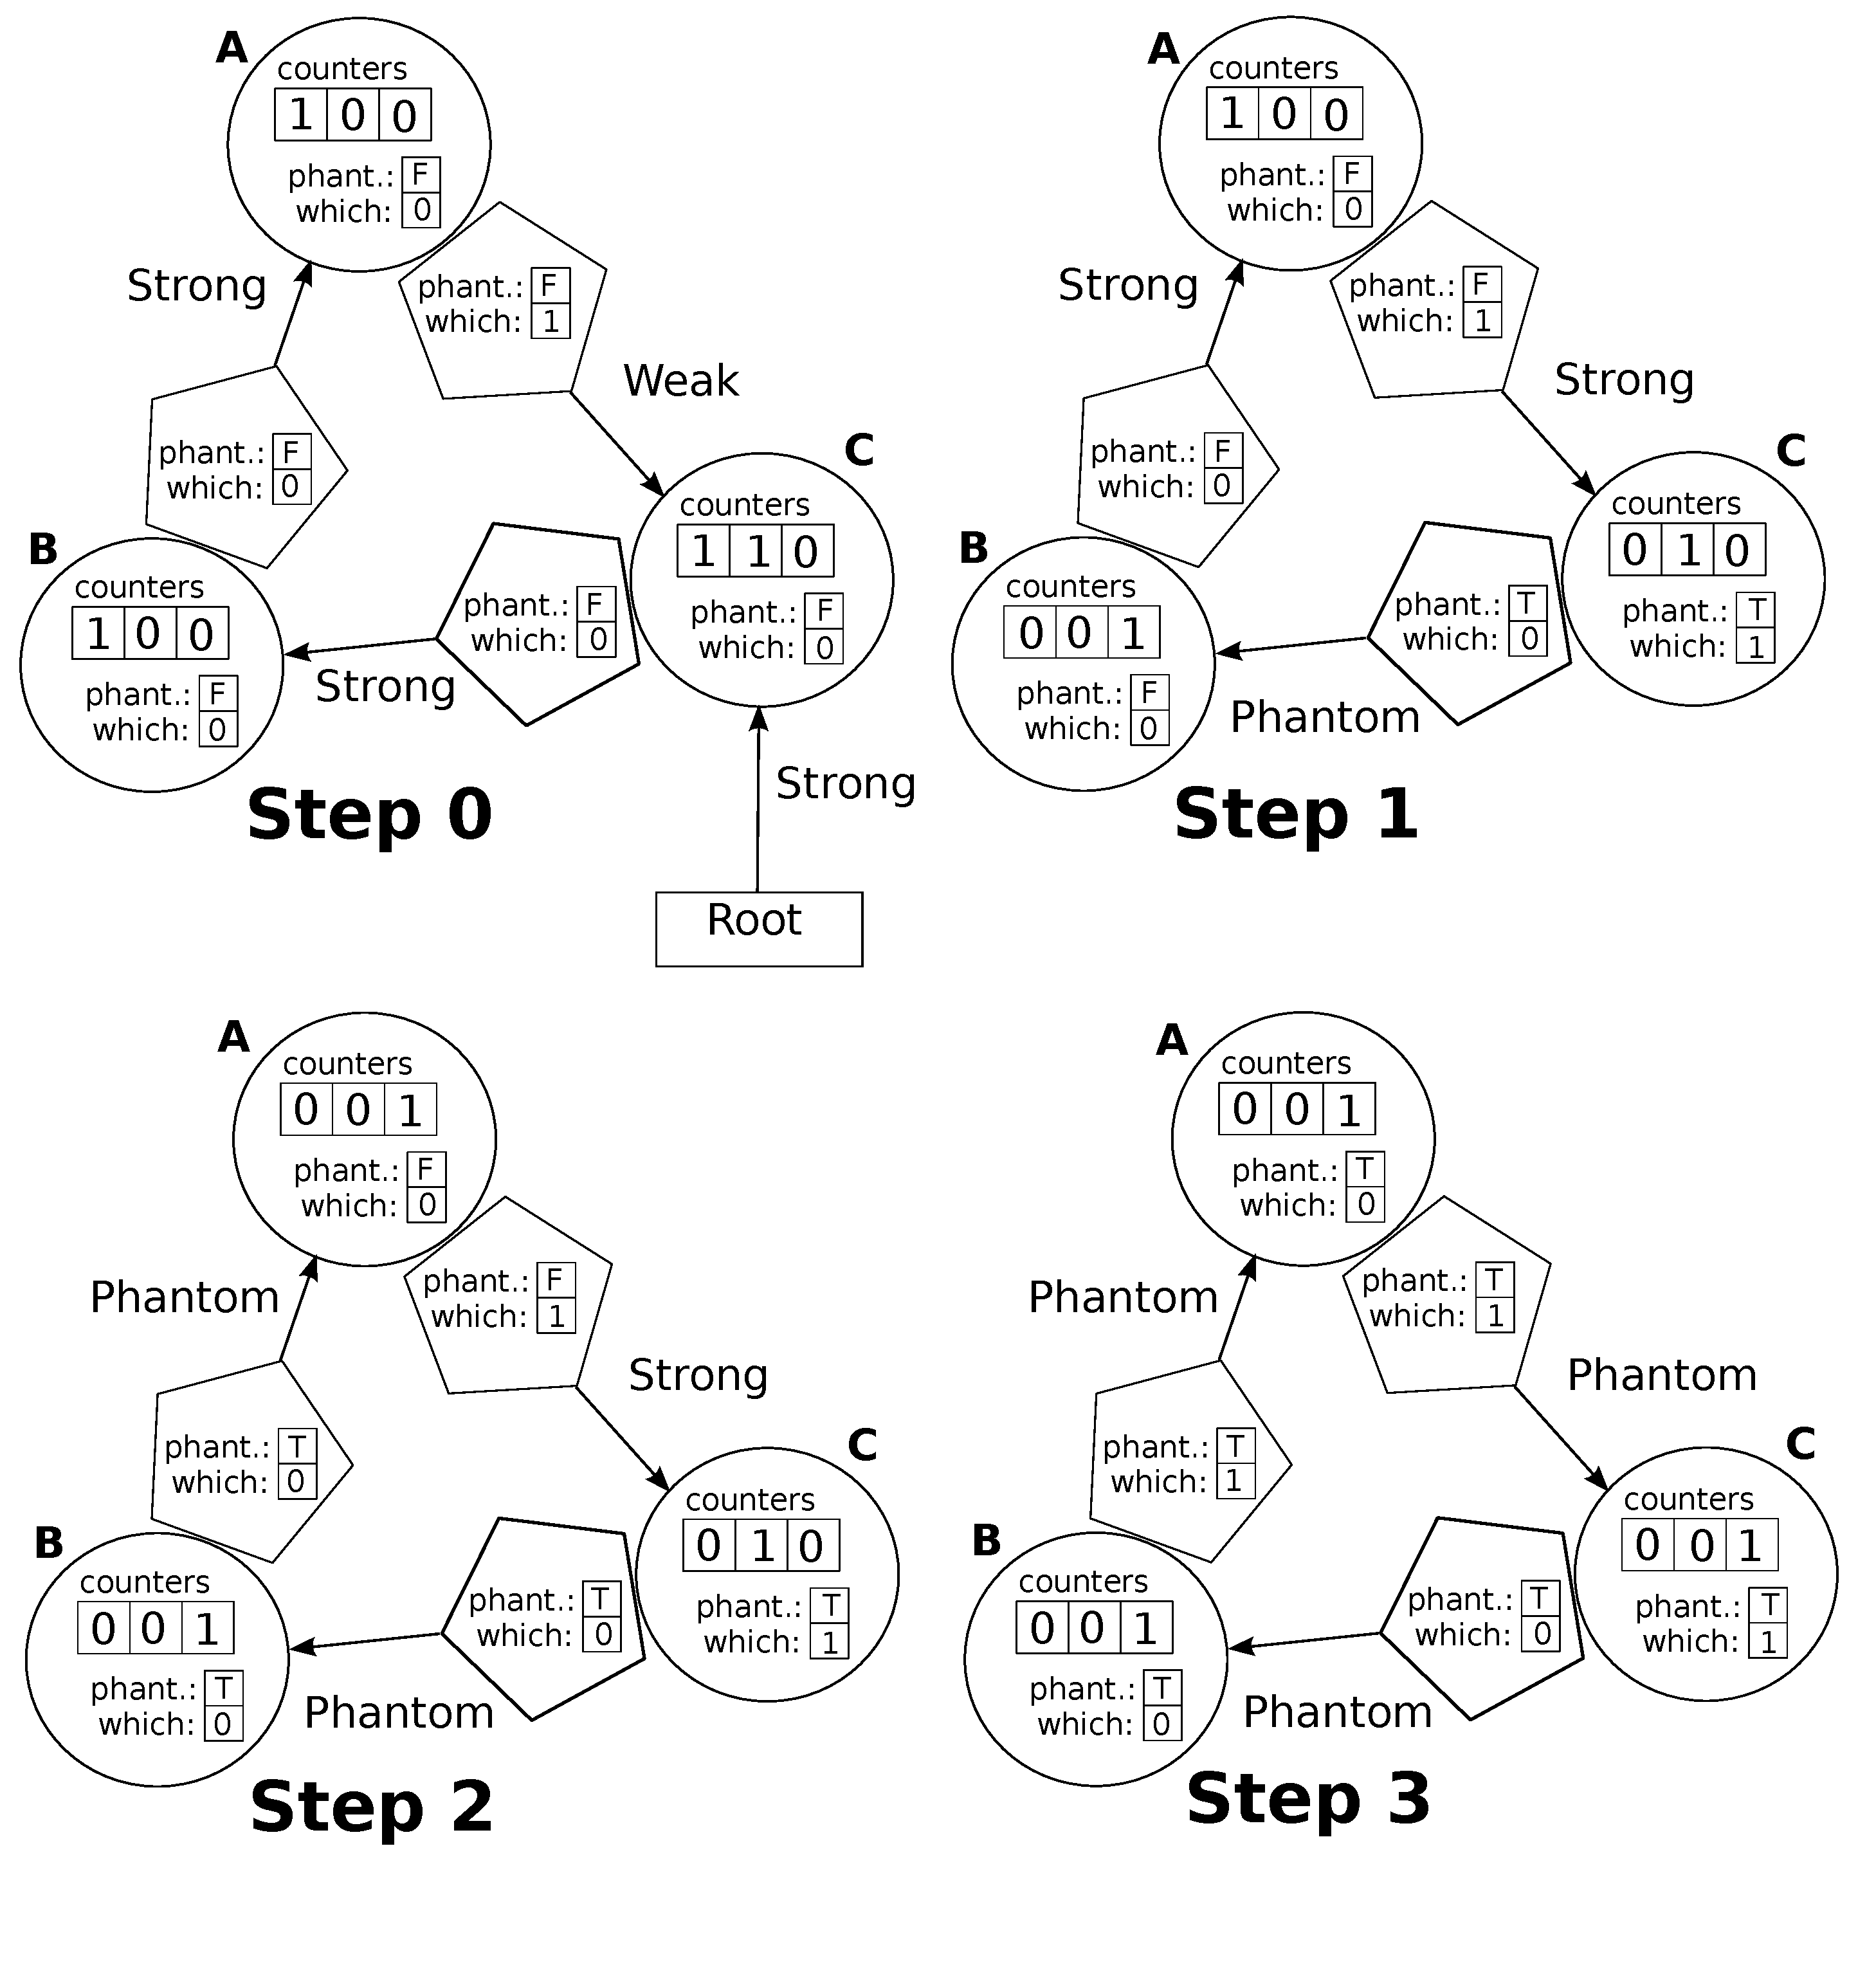
\includegraphics[width=0.5\textwidth]{figs/method}
%\caption{Reclaiming a cycle with three objects.}
%\label{ex1}
%\end{figure}

\begin{figure*}[!t]
  \centering
  %\subfloat[Initially, the owner node $v$ publishes the object]
  {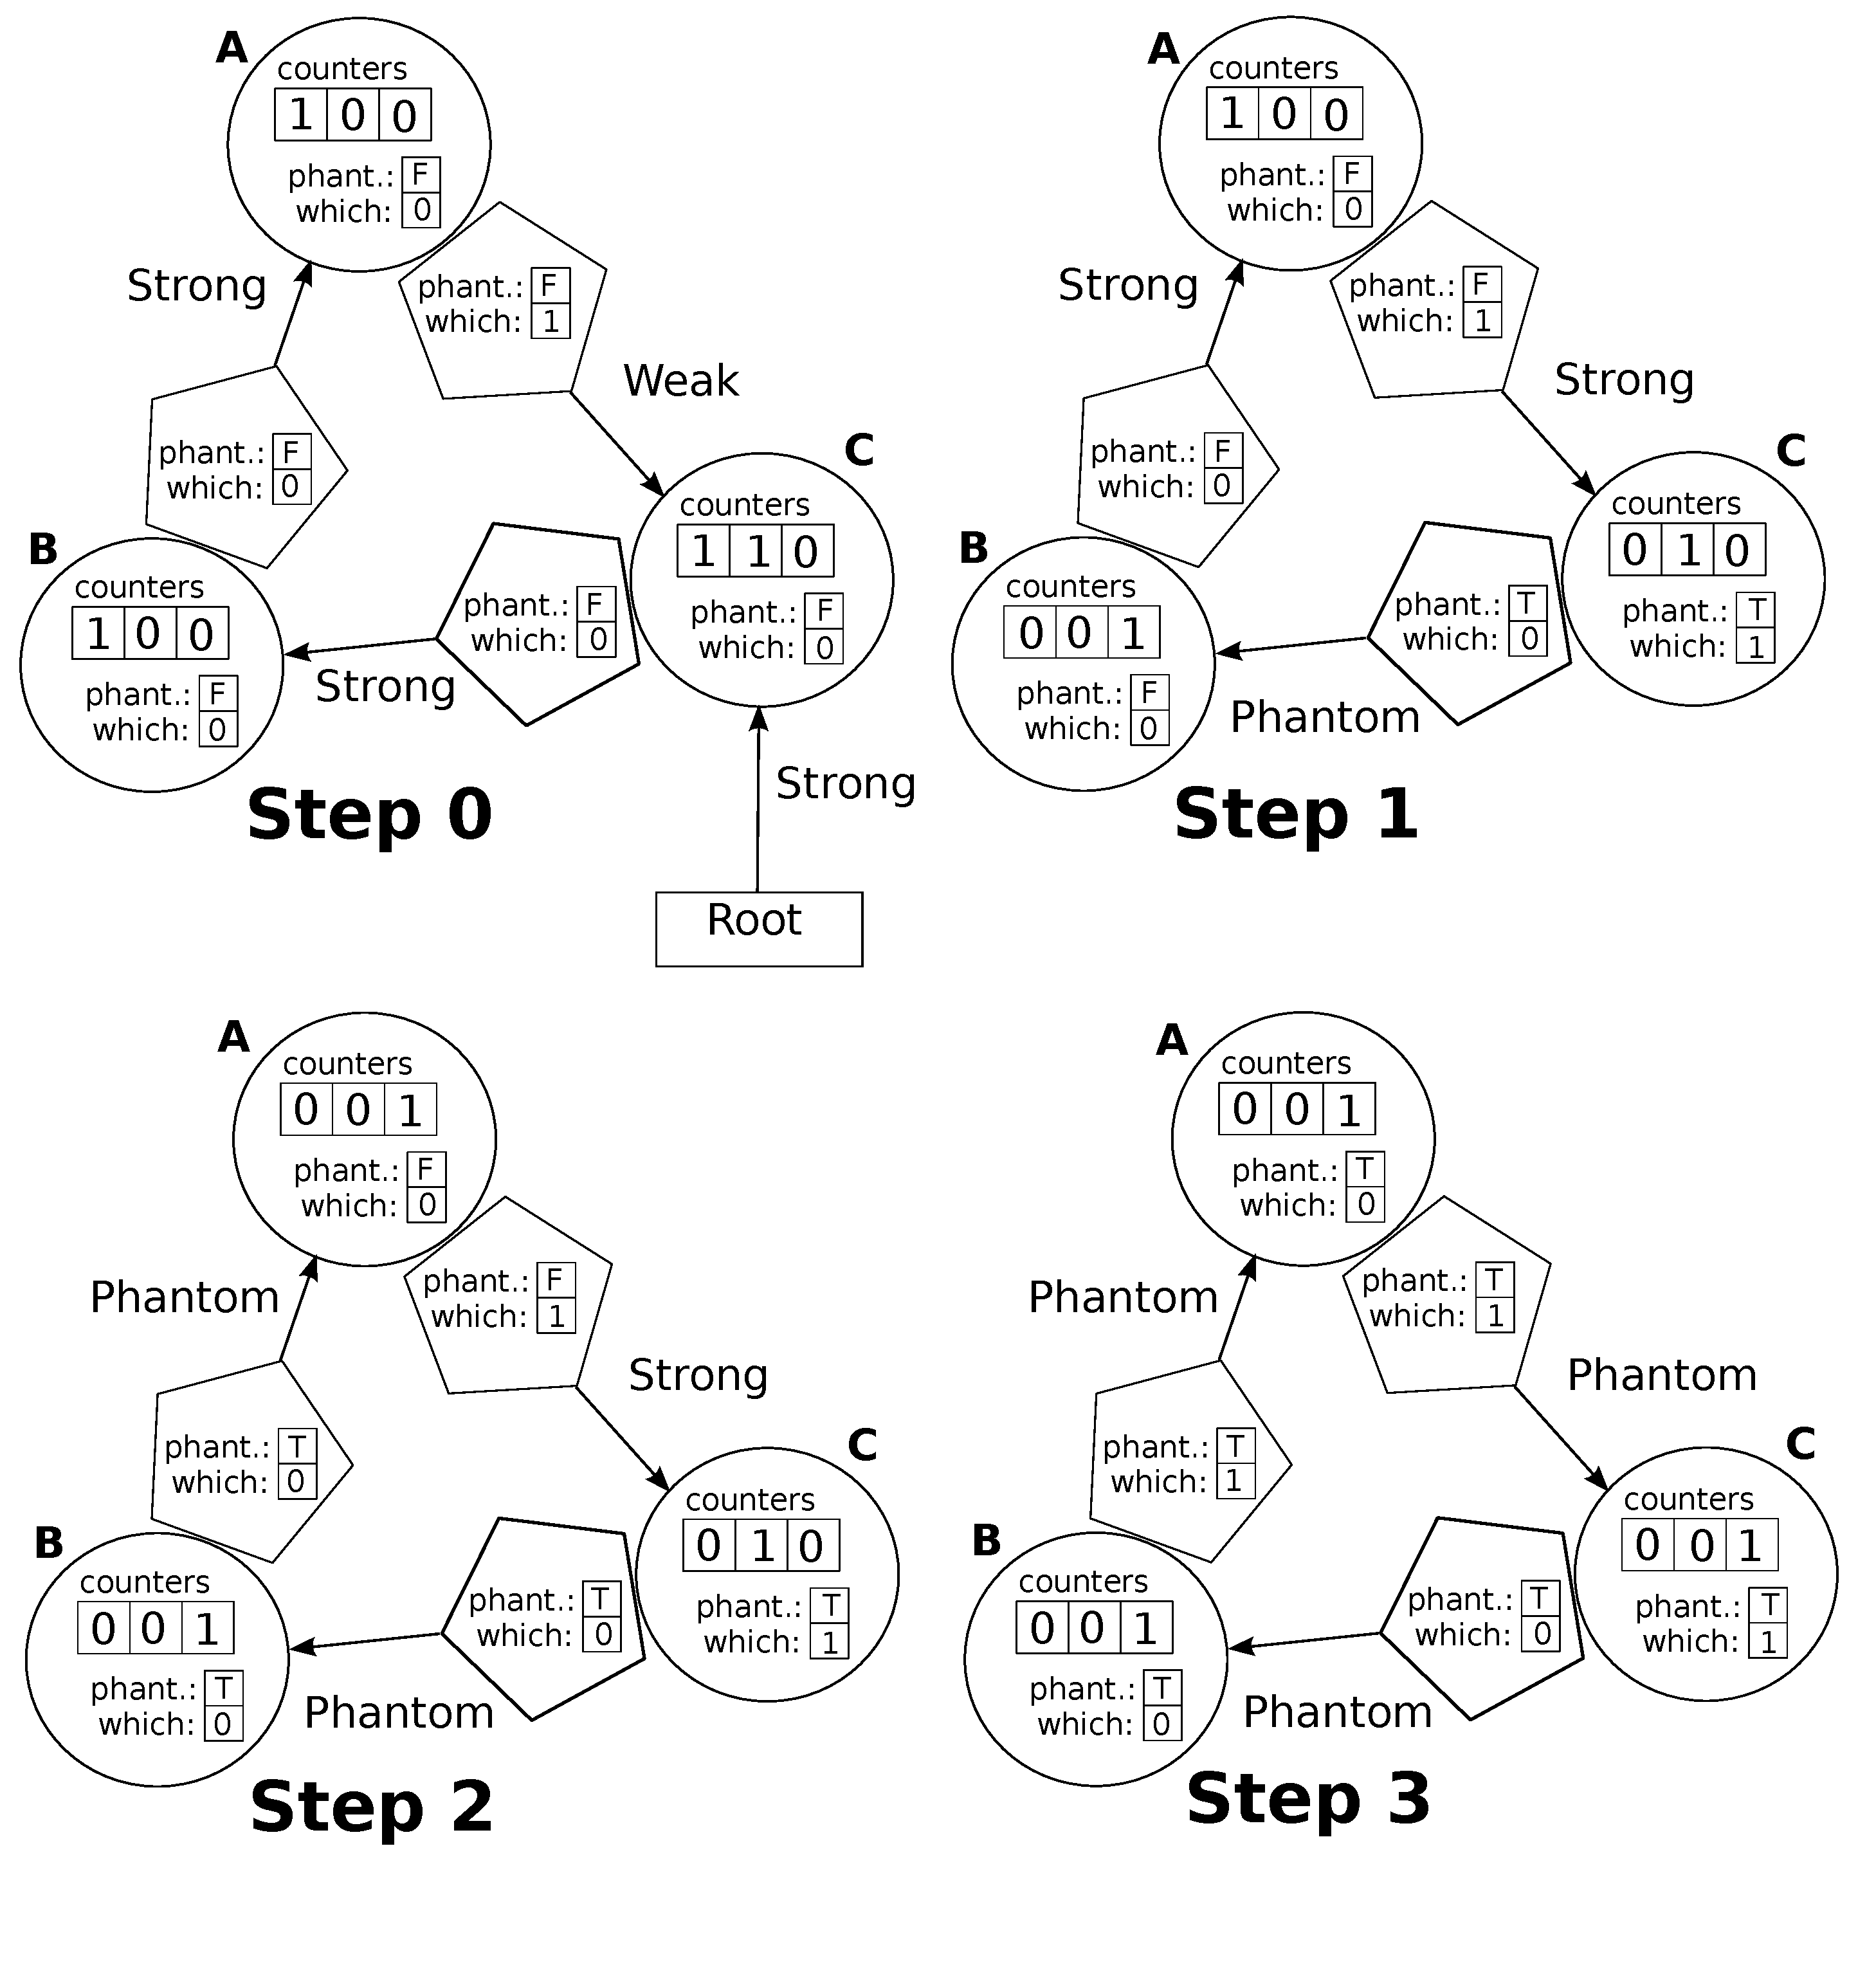
\includegraphics[height=4.5in]{figs/method}\label{fig:example1}}
  %\hspace{30pt}%
  %\subfloat[Node $u$ issues a ${\sf move}$ request]
  %{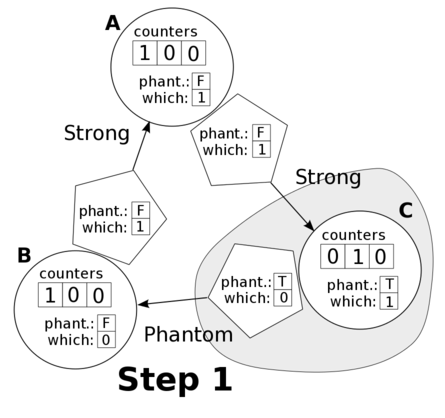
\includegraphics[height=2.0in]{figs/method1}\label{fig:example2}}\\
  %\hspace{12pt}%
  %\subfloat[The request continues up phase]
  %{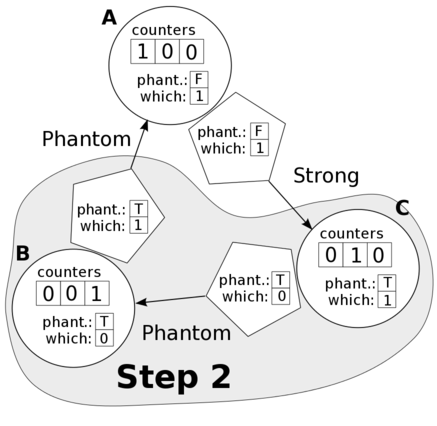
\includegraphics[height=2.0in]{figs/method2}\label{fig:example3}}
  %\hspace{30pt}%
  %\subfloat[Directory path found, new owner node $u$]
  %{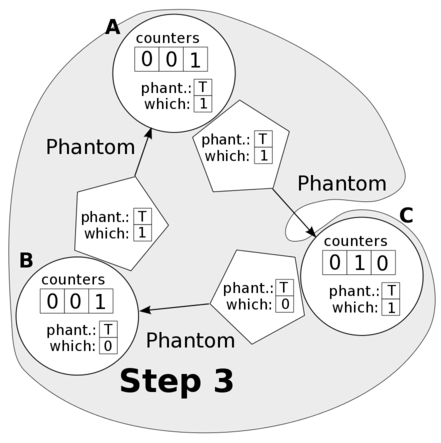
\includegraphics[height=2.0in]{figs/method3}\label{fig:example4}}
  \caption{Reclaiming a cycle with three objects}%
  \label{ex1}
\end{figure*}

\begin{figure*}[!t]
  \centering
  %\subfloat[Initially, the owner node $v$ publishes the object]
  {\includegraphics[height=2.0in]{figs/doublylinkedlist}\label{fig:example2}}
 \caption{Doubly-linked list}%
  \label{ex2}
\end{figure*}

%\begin{figure}
%\centering
%\begin{minipage}{.167\textwidth}
%    \centering
%    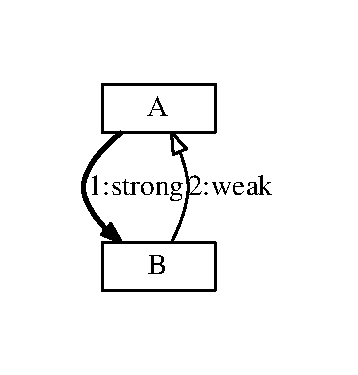
\includegraphics[width=1.0\textwidth]{figs/ex1step0}
%    %\caption{ }
%\end{minipage}%
%\begin{minipage}{.166\textwidth}
%    \centering
%    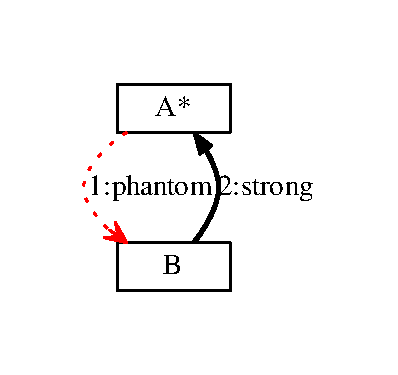
\includegraphics[width=1.0\textwidth]{figs/ex1step1}
%    %\caption{ }
%\end{minipage}%
%\begin{minipage}{.167\textwidth}
%    \centering
%    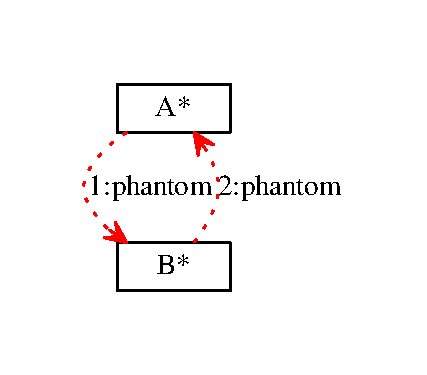
\includegraphics[width=1.0\textwidth]{figs/ex1step2}
%    %\caption{ }
%\end{minipage}%
%\end{figure}


\begin{comment}
\begin{figure}
\centering
\begin{minipage}{.167\textwidth}
    \centering
    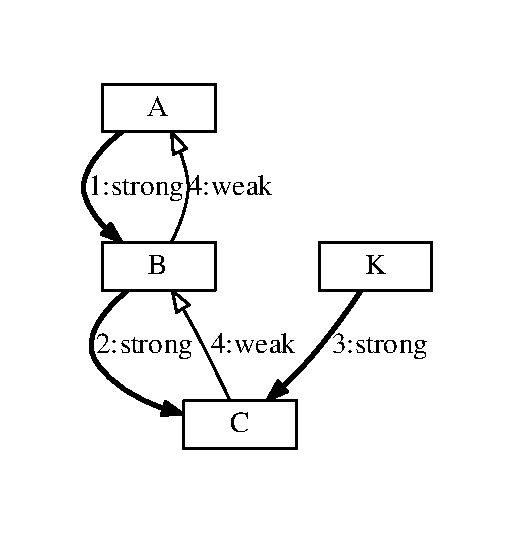
\includegraphics[width=1.0\textwidth]{figs/ex3step0}
    %\caption{ }
\end{minipage}%
\begin{minipage}{.166\textwidth}
    \centering
    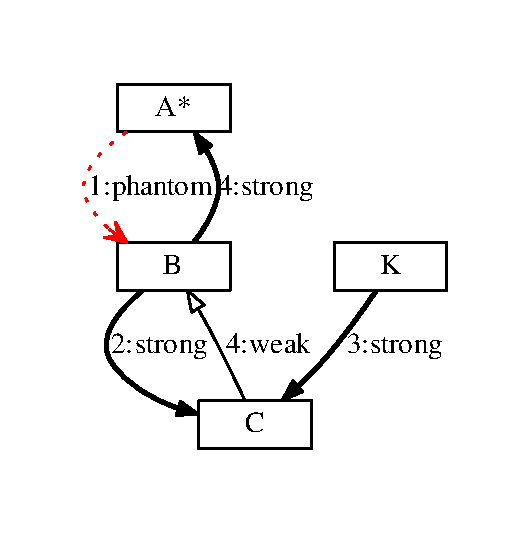
\includegraphics[width=1.0\textwidth]{figs/ex3step1}
    %\caption{ }
\end{minipage}%
\begin{minipage}{.167\textwidth}
    \centering
    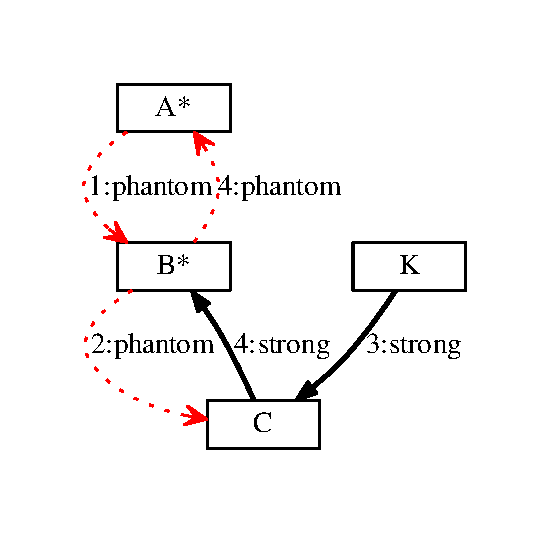
\includegraphics[width=1.0\textwidth]{figs/ex3step2}
    %\caption{ }
\end{minipage}

\begin{minipage}{.167\textwidth}
    \centering
    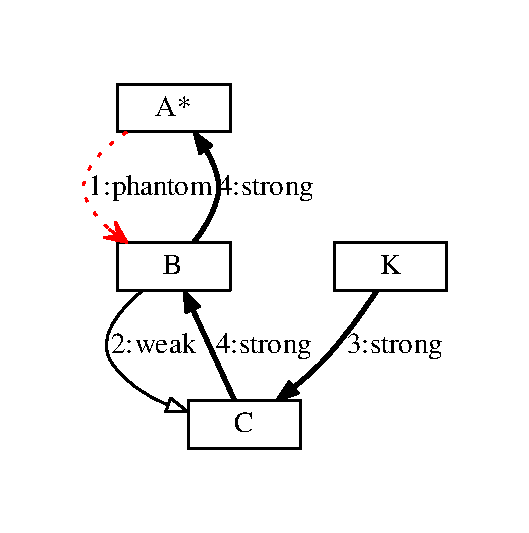
\includegraphics[width=1.0\textwidth]{figs/ex3step3}
    %\caption{ }
\end{minipage}%
\begin{minipage}{.166\textwidth}
    \centering
    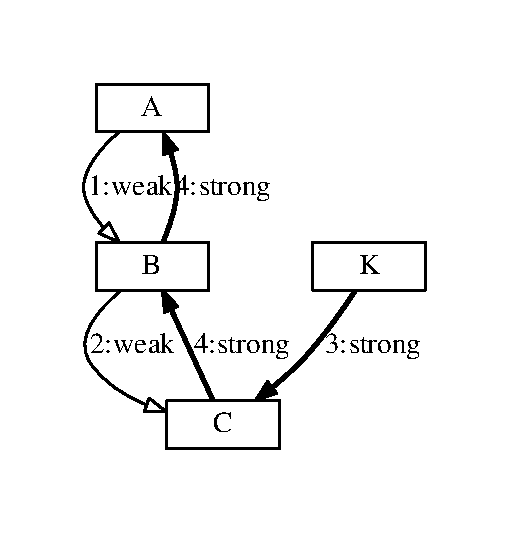
\includegraphics[width=1.0\textwidth]{figs/ex3step4}
    %\caption{ }
\end{minipage}%
\label{ex3}
\caption{Rebalancing a Doubly-Linked List}
\end{figure}
\end{comment}


\begin{figure*}[!t]
  \centering
  %\subfloat[Initially, the owner node $v$ publishes the object]
  {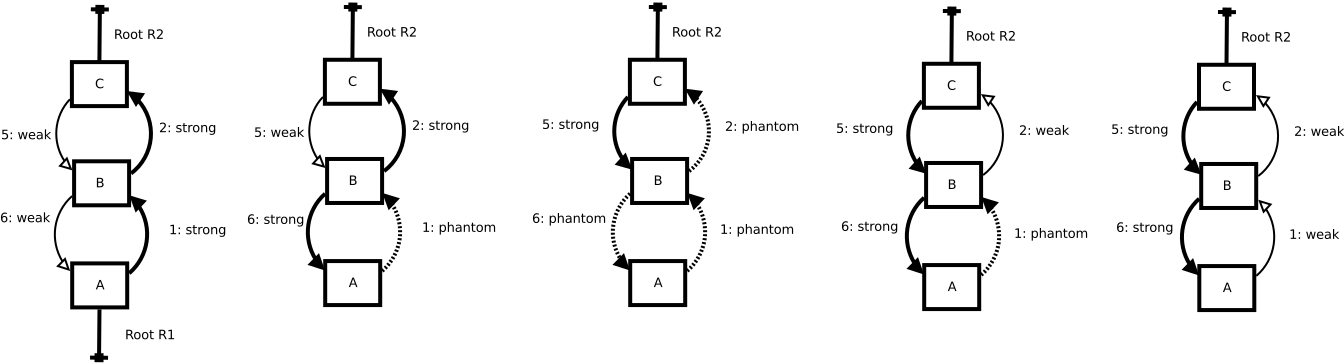
\includegraphics[height=2.0in]{figs/recoveringdbl}}%\label{fig:example1}}

  \caption{Rebalancing a doubly-linked list}%
  \label{ex3}
\end{figure*}


\subsection{Example: A Doubly-Linked List}

The doubly linked list depicted in Fig.~\ref{ex2} is a classic
example for garbage collection systems. The structure consists of
6 links, and the collector marks all the links as phantoms in 8
steps.

This figure contains much less detail than Fig.~\ref{ex1}, which
is necessary for a more complex figure.

%There are several options to choose from in deciding
%how to represent this particular structure in memory, but this
%example should suffice to enable the reader to work
%through additional similar examples.

% \begin{comment}
% \begin{figure}
% \centering
% \begin{minipage}{.167\textwidth}
%     \centering
%     \includegraphics[width=1.0\textwidth]{figs/doublylinkedlist}
%     %\caption{ }
% \end{minipage}%
%\begin{minipage}{.167\textwidth}
%   \centering
%    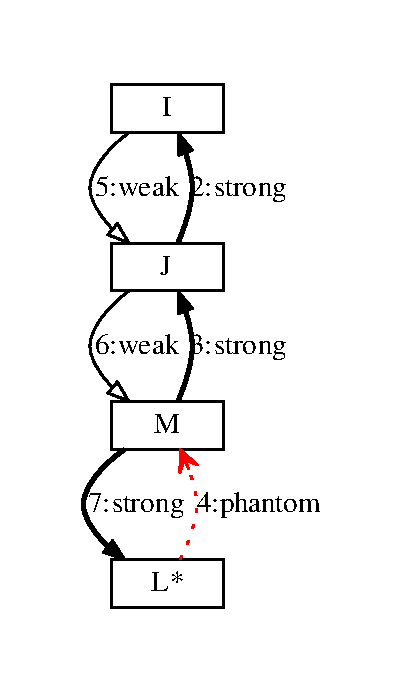
\includegraphics[width=1.0\textwidth]{figs/ex2step1}
%    %\caption{ }
%\end{minipage}%
%\begin{minipage}{.166\textwidth}
%    \centering
%    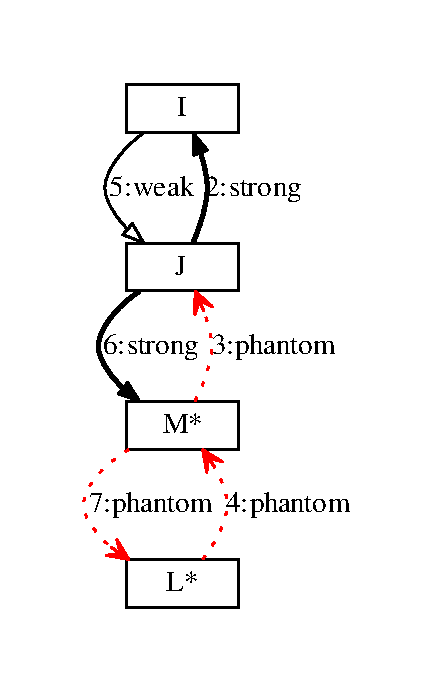
\includegraphics[width=1.0\textwidth]{figs/ex2step2}
%    %\caption{ }
%\end{minipage}

%\begin{minipage}{.167\textwidth}
%    \centering
%    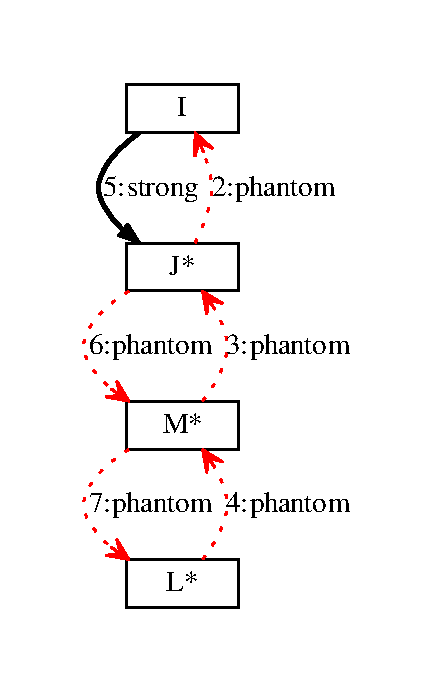
\includegraphics[width=1.0\textwidth]{figs/ex2step3}
%    %\caption{ }
%\end{minipage}%
%\begin{minipage}{.167\textwidth}
%    \centering
%    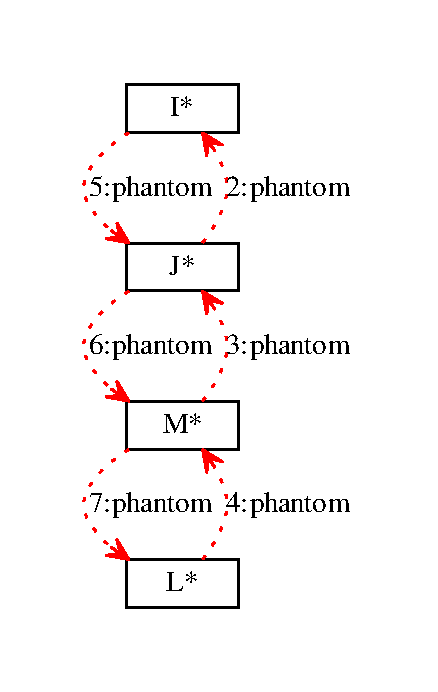
\includegraphics[width=1.0\textwidth]{figs/ex2step4}
%    %\caption{ }
%\end{minipage}%
%\label{ex2}
%\caption{Reclaiming a double cycle.}
% \end{figure}
% \end{comment}

% \begin{figure*}[!t]
%   \centering
%   %\subfloat[Initially, the owner node $v$ publishes the object]
%   {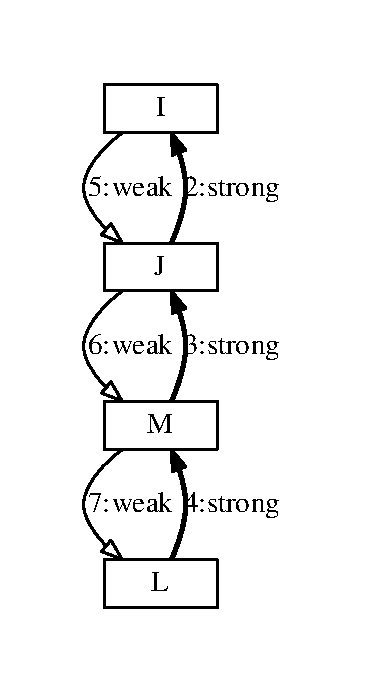
\includegraphics[height=1.6in]{figs/ex2step0}}%\label{fig:example1}}
%   \hspace{12pt}%
%   %\subfloat[Node $u$ issues a ${\sf move}$ request]
%   {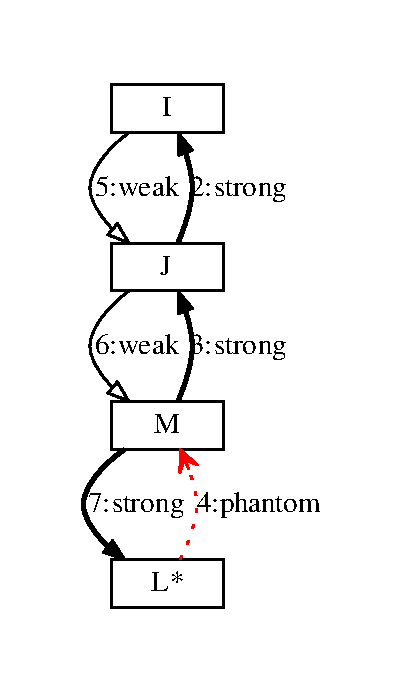
\includegraphics[height=1.6in]{figs/ex2step1}}%\label{fig:example2}}
%   \hspace{12pt}%
%   %\subfloat[The request continues up phase]
%   {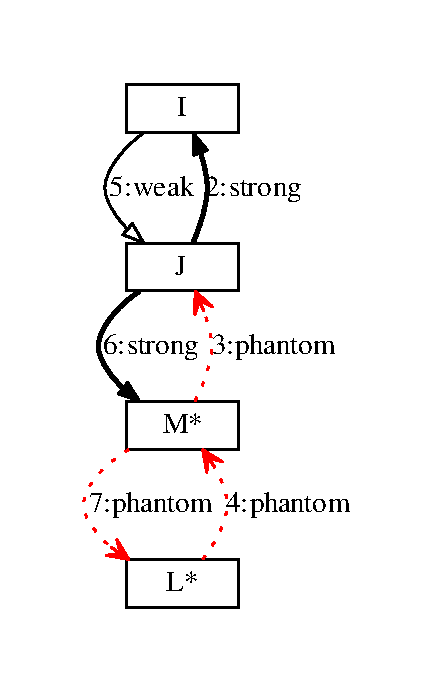
\includegraphics[height=1.6in]{figs/ex2step2}}%\label{fig:example3}}
%   \hspace{12pt}%
%   %\subfloat[Directory path found, new owner node $u$]
%   {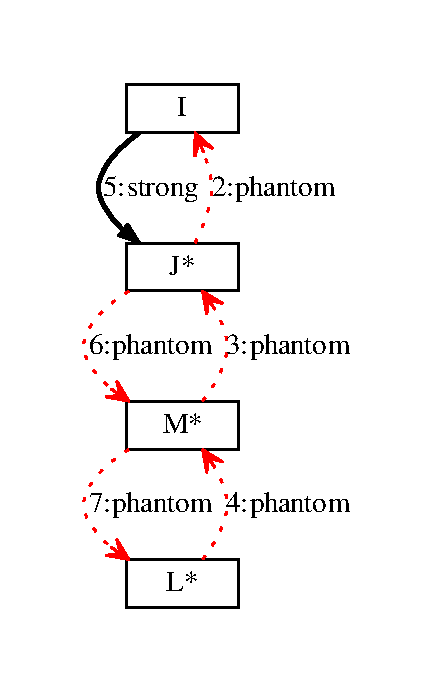
\includegraphics[height=1.6in]{figs/ex2step3}}%\label{fig:example4}}
%   \hspace{12pt}%
%   %\subfloat[Directory path found, new owner node $u$]
%   {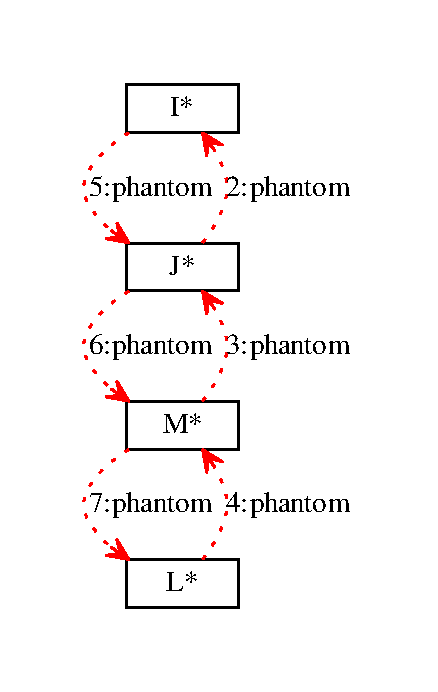
\includegraphics[height=1.6in]{figs/ex2step4}}%\label{fig:example4}}
%   \caption{Reclaiming a double cycle}%
%   \label{ex2}
% \end{figure*}

\subsection{Example: Rebalancing A Doubly-Linked List}

Fig.~\ref{ex3} represents a worst case scenario for our algorithm. As a
result of losing root $R1$, the
strong links are pointing in exactly the wrong direction to provide
support across
an entire chain of double links. During $Phantomization$, each
of the objects in the list must convert its links to phantoms,
but nothing is deleted. $Phantomization$ is complete in the third
figure from the left, and $Recovery$ begins.
The fourth step in the figure, when link 6 is converted from phantom to weak
marks the first phase of the recovery.



\subsection{Example: Recovering Without Detecting a Cycle}

In Fig.~\ref{prove} we see the situation where the collector recovers from the
loss of a strong link without searching the entire cycle. When root $R1$ is removed,
node $A$ becomes phantomized. It turns its incoming link (link $1$) to strong,
and phantomizes its outgoing link (link $2$), but
then the phantomization process ends. Recovery is successful, because $A$ has strong
support, and it rebuilds its outgoing link as weak. At this point, collection
operations are finished.

Unlike the doubly-linked list example above, this case describes an optimal
situation for our garbage collection system.

\section{Concurrency Issues}

%Note that the algorithm section omits the actual calls to lock and unlock present in our fine-grained parallel prototype.
This section provides details of the implementation.
%A reference implementation is also provided ~\cite{url:refimpl}.\todo{Make public repo}
%\update{What about we provide implementation link here. Currently it is withheld for supporting double-blind review. I think the link will make our case stronger and it does not reveal our identity directly.}

\subsection{The Single-Threaded Collector}
There are several methods by which the collector may be
allowed to interact concurrently with a live system. The first, and most straightforward
implementation, is to use a single garbage collection thread to manage nontrivial
collection operations. This technique has the advantage of limiting the amount
of computational power the garbage collector may use to perform its work.

For the collection process to work, phantomization must run to completion before
recovery is attempted, and recovery must run to completion before cleanup can
occur. To preserve this ordering in a live system,
whenever an operation would remove the last strong link
to an object with weak or phantom references, the link is instead transferred
to the collector, enabling it to perform phantomization at an appropriate time.
%See Algorithms.~\ref{algorithm:linkfree} and~\ref{algorithm:addtocollector}.

%In Algorithm~\ref{algorithm:addtocollector}, we see that
After the strong link is processed, the garbage collector needs to create a phantom
link to hold onto the object while it performs its processing, to ensure the
collector itself doesn't try to use a deleted object.

Another point of synchronization is the creation of new links. If the
source of the link is a phantomized node, the link is created in the phantomized
state. %See Algorithm~\ref{algorithm:linkset}.

With these relatively straightforward changes, the single-threaded garbage collector
may interact freely with a live system.

%Note that in the following sections, locks are always obtained in canonical order that avoids deadlocks. Unlock methods unlock the last set of items that were locked.

The lists on the collectors are thread-safe.

The collector object is itself managed by a simple reference count. Code for incrementing and decrementing this count is not explicitly present in the code below.

A reference implementation is also provided ~\cite{url:refimpl}.

\begin{algorithm}[ht]
{\small
\tcp{LinkSet creates a new link,
  and decides the type of the link to create.}
{\bf LinkSet(link,node)}:\\
\quad {lock (link.Source,node)}\\
\quad {\bf if} node == NULL {\bf then}\\
\quad \quad LinkFree(link)\\
\quad \quad link.Target = NULL\\
\quad {\bf EndIf}\\
\quad {\bf if} link.Target == node {\bf then}\\
\quad \quad {\bf Return}\\
\quad {\bf EndIf}\\
\quad oldLink = copy(link) \\
\quad link.Target = node\\
\quad {\bf If} link.Source.Phantomized {\bf then}\\
\quad \quad MergeCollectors(link.Source, link.Target)\\
\quad \quad link.PhantomCount++\\
\quad \quad link.Phantomized = True\\
\quad {\bf ElseIf} link.Source == node {\bf then}\\
\quad \quad link.Which = 1 - node.Which\\
\quad \quad node.Count[link.Which]++\\
\quad {\bf ElseIf} node.Links not initialized {\bf then}\\
\quad \quad node.Count[link.Which]++\\
\quad \quad link.Which = node.Which\\
\quad {\bf Else}\\
\quad \quad link.which = 1 - node.Which\\
\quad \quad node.Count[link.Which]++\\
\quad {\bf EndIf}\\
\quad {\bf If} oldLink != NULL\\
\quad \quad LinkFree(oldLink)\\
\quad  {unlock()}\\
}
\caption{LinkSet}
\label{single:algorithm:linkset}
\end{algorithm}
\setlength{\textfloatsep}{0pt}
\begin{algorithm}[ht]
{\small
\tcp{Freeing a link is usually just the decrement of a reference count, but
if it is the last strong count, this could potentially start a Phantomization process.}
%\begin{multicols}{2}
% \tcp{$R$ and $S$ are objects currently in use.}
{\bf LinkFree(link)}:\\
% \tcp*[f]{Create a pointer from object $R$ to some free object}\\
{\Indp
{lock(link.Source,link.Target)}\\
{\bf If} link.Target == NULL {\bf then}\\
\quad {\bf Return}\\
{\bf EndIf}\\
{\bf If} link.Phantomized {\bf then}\\
\quad DecPhantom(link.Target)\\
{\bf Else}\\
\quad link.Target.Count[link.Which]-\,-\\
\quad {\bf If} link.Target.Count[link.Which] == 0 {\bf And} \\
\quad \quad \quad link.Target.Which == link.Which {\bf then}\\
\quad \quad {\bf If} link.Target.Count[1-link.Target.Which] == 0 {\bf And} \\
\quad \quad \quad \quad link.Target.PhantomCount == 0 {\bf then}\\
\quad \quad \quad Delete(node)\\
\quad \quad \quad link.Target = NULL\\
\quad \quad {\bf Else} \\
\quad \quad \quad {\bf If} link.Target.Collector == NULL {\bf then}\\
\quad \quad \quad \quad link.Target.Collector = new Collector()\\
\quad \quad \quad {\bf EndIf}\\
\quad \quad \quad AddToCollector(link.Target)\\
\quad \quad {\bf EndIf} \\
\quad {\bf EndIf}\\
{\bf EndIf}\\
{unlock()}\\
}
}
\caption{LinkFree}
\label{algorithm:linkfree}
\end{algorithm}
\setlength{\textfloatsep}{0pt}
\begin{algorithm}[ht]
{\small
%\begin{multicols}{2}
% \tcp{$R$ and $S$ are objects currently in use.}
% \tcp*[f]{Create a pointer from object $R$ to some free object}\\
\tcp{Adding an object to the collector puts back the strong
count, effectively transferring the source of the strong link
to the collector. It also adds a phantom count, which helps
prevent the clearing of the Collector field.}
{\bf AddToCollector(node)}:\\
{\Indp
{\bf While} True\\
\quad {lock(node,node.Collector)}\\
\quad {\bf If} node.Collector.Forward != NULL {\bf then}\\
\quad \quad node.Collector = node.Collector.Forward\\
\quad {\bf Else}\\
\quad \quad node.Count[node.Which]++\\
\quad \quad node.PhantomCount++\\
\quad \quad node.Collector.CollectionList.append(node)\\
\quad \quad {\bf Break}\\
\quad {\bf EndIf}\\
\quad {unlock()}\\
{\bf EndWhile}\\
}
}
\caption{AddToCollector}
\label{single:algorithm:addtocollector}
\end{algorithm}
%\end{multicols}
\setlength{\textfloatsep}{0pt}
\begin{algorithm}[ht]
{\small
%\begin{multicols}{2}
\tcp{The collector takes away the strong link it made in
AddToCollector().
}
{\bf PhantomizeNode(node,collector)}:\\
{\Indp
{lock(node)}\\
{\bf While} collector.Forward != NULL\\
\quad collector = collector.Forward\\
{\bf EndWhile}\\
node.Collector = collector\\
node.Count[node.Which]-\,-\\
\quad // Prevent deletion while the\\
\quad // node is managed by the Collector\\
{\bf Let} phantomize = False\\
{\bf If} node.Count[node.Which] $>$ 0 {\bf then}\\
\quad {\bf Return}\\
{\bf Else}\\
\quad {\bf If} node.Count[1-node.Which] $>$ 0 {\bf then}\\
\quad \quad node.Which = 1-node.Which\\
\quad {\bf EndIf}\\
\quad {\bf If} {\bf Not} node.Phantomized {\bf then}\\
\quad \quad node.Phantomized = True\\
\quad \quad node.PhantomizationComplete = False\\
\quad \quad phantomize = True\\
\quad {\bf EndIf}\\

{\bf EndIf}\\
{\bf Let} links = NULL \\
{\bf If} phantomize {\bf then}\\
\quad links = copy(node.Links)\\
{\bf EndIf}\\
{unlock()}\\
{\bf ForEach} outgoing link in links\\
\quad PhantomizeLink(link)\\
{\bf EndFor}\\
lock(node)\\
{node.PhantomizationComplete = True}\\
unlock()\\
}
%\end{multicols}
}
\caption{PhantomizeNode}
\label{algorithm:phantomizenode}
\end{algorithm}
\setlength{\textfloatsep}{0pt}
\begin{algorithm}[ht]
{\small
%\begin{multicols}{2}
\tcp{This method describes the
work to be carried out by a
garbage collection thread. Live
objects pointing to this collector, or
Forward pointers from other collectors
contribute to the RefCount field on
the Collector.}
{\bf Collector.Main()}:\\
{\Indp
{\bf While} True \\
\quad WaitFor(Collector.RefCount == 0 {\bf Or} Work to do)\\
\quad {\bf If} Collector.RefCount == 0 {\bf And} No work to do {\bf then}\\
\quad \quad {\bf Break}\\
\quad {\bf EndIf}\\
\quad {\bf While} Collector.MergedList.size() $>$ 0\\
\quad \quad Let node = Collector.MergedList.pop()\\
\quad \quad Collector.RecoveryList.append(node)\\
\quad {\bf EndWhile}\\
\quad {\bf While} Collector.CollectionList.size() $>$ 0\\
\quad \quad Let node = Collector.CollectionList.pop()\\
\quad \quad PhantomizeNode(node,Collector)\\
\quad \quad Collector.RecoveryList.append(node)\\
\quad {\bf EndWhile}\\
\quad {\bf While} Collector.RecoveryList.size() $>$ 0\\
\quad \quad Let node = Collector.RecoveryList.pop()\\
\quad \quad RecoverNode(node)\\
\quad \quad Collector.CleanList.append(node)\\
\quad {\bf EndWhile}\\
\quad {\bf While} Collector.RebuildList.size() $>$ 0\\
\quad \quad Let node = Collector.RebuildList.pop()\\
\quad \quad RecoverNode(node)\\
\quad {\bf EndWhile}\\
\quad {\bf While} Collector.CleanList.size() $>$ 0\\
\quad \quad Let node = Collector.CleanList.pop()\\
\quad \quad CleanNode(node)\\
\quad {\bf EndWhile}\\
{\bf EndWhile}\\
}
}
\caption{Collector.Main}
\label{algorithm:main}
\end{algorithm}
\setlength{\textfloatsep}{0pt}
\begin{algorithm}[ht]
{\small
%\begin{multicols}{2}
{\bf PhantomizeLink(link)}:\\
{\Indp
 {lock(link.Source,link.Target)}\\
 {\bf If} link.Target == NULL {\bf then}\\
\quad  {unlock()}\\
 \quad {\bf Return}\\
 {\bf EndIf}\\
{\bf If} link.Phantomized {\bf then}\\
\quad  {unlock()}\\
\quad {\bf Return} \\
{\bf EndIf}\\
link.Target.PhantomCount++\\
link.Phantomized = True\\
linkFree(link)\\
MergeCollectors(link.Source, link.Target)\\
 {unlock()}\\
}
}
\caption{PhantomizeLink}
\label{single:algorithm:phantomizelink}
\end{algorithm}
\setlength{\textfloatsep}{0pt}
\begin{algorithm}[ht]
{\small
%\begin{multicols}{2}
\tcp{DecPhantom is responsible for removing any reference to
the collector.}
{\bf DecPhantom(node)}:\\
{\Indp
 {lock(node)}\\
node.PhantomCount- -\\
{\bf If} node.PhantomCount == 0 {\bf then}\\
\quad {\bf If} node.Count[node.Which]== 0 {\bf And}\\
\quad \quad \quad node.Count[1-node.Which] == 0 {\bf then}\\
\quad \quad Delete(node)\\
\quad {\bf Else}\\
\quad \quad node.Collector = NULL\\
\quad {\bf EndIf}\\
{\bf EndIf}\\
 {unlock()}\\
}
}
\caption{DecPhantom}
\label{single:algorithm:decPhantom}
\end{algorithm}
\setlength{\textfloatsep}{0pt}

\begin{algorithm}[ht]
{\small
%\begin{multicols}{2}
{\bf RecoverNode(node)}:\\
{\Indp
 {lock(node)}\\
{\bf Let} links = NULL\\
{\bf If} node.Count[node.Which] $>$ 0 {\bf then}\\
\quad WaitFor(node.PhantomizationComplete == True)\\
\quad node.Phantomized = False\\
\quad links = copy(node.Links)\\
{\bf EndIf}\\
 {unlock()}\\
{\bf ForEach} link in links \\
\quad Rebuild(link)\\
{\bf EndFor}\\
}
}
\caption{RecoverNode}
\label{algorithm:recover}
\end{algorithm}
\setlength{\textfloatsep}{0pt}

\begin{algorithm}[ht]
{\small
%\begin{multicols}{2}
{\bf Rebuild(link)}:\\
{\Indp
 {lock(link.Source,link.Target)}\\
{\bf If} link.Phantomized {\bf then}\\
\quad {\bf If} link.Target == link.Source {\bf then}\\
\quad \quad link.Which = 1- link.Target.Which\\
\quad {\bf ElseIf} link.Target.Phantomized {\bf then} \\
\quad \quad link.Which = link.Target.Which\\
\quad {\bf ElseIf} count(link.Target.Links) == 0 {\bf then}\\
\quad \quad link.Which = link.Target.Which\\
\quad {\bf Else}\\
\quad \quad link.Which = 1-link.Target.Which\\
\quad {\bf EndIf}\\
\quad link.Target.Count[link.Which]++\\
\quad link.Target.PhantomCount- -\\
\quad{\bf If} link.Target.PhantomCount == 0 {\bf then}\\
\quad \quad link.Target.Collector = NULL\\
\quad {\bf EndIf}\\
\quad link.Phantomized = False \\
\quad Add link.Target to Collector.RecoveryList\\
{\bf EndIf}\\
 {unlock()}\\
}
}
\caption{Rebuild}
\label{single:algorithm:rebuild}
\end{algorithm}
\setlength{\textfloatsep}{0pt}

\begin{algorithm}[ht]
{\small
%\begin{multicols}{2}
\tcp{After deleting all the outgoing links, decrement
the phantom count by one (i.e. the reference held by
the collector itself). When the last phantom count
is gone, the object is cleaned up.}
{\bf  CleanNode(node)}:\\
{\Indp
 {lock(node)}\\
{\bf Let} die = False\\
{\bf If} node.Count[node.Which]== 0 {\bf And}\\
\quad \quad node.Count[1-node.Which]== 0 {\bf then}\\
\quad  die = True\\
{\bf EndIf}\\
{unlock()}\\
{\bf If} die {\bf then}\\
\quad {\bf ForEach} link in node\\
\quad \quad LinkFree(link)\\
\quad {\bf EndFor}\\
{\bf EndIf}\\
DecPhantom(node)\\
 }
}
\caption{CleanNode}
\label{algorithm:cleanup}
\end{algorithm}
\setlength{\textfloatsep}{0pt}
\begin{algorithm}[ht]
{\small
{\bf  Delete(node)}:\\
{\Indp
\quad {\bf ForEach} link in node \\
\quad \quad LinkFree(link)\\
\quad {\bf EndFor}\\
\quad freeMem(node)\\

 }
}
\caption{Delete}
\label{algorithm:Delete}
\end{algorithm}
\setlength{\textfloatsep}{0pt}

\begin{algorithm}[ht]
{\small
%\begin{multicols}{2}
\tcp{When two collector threads
realize they are managing a common
subset of objects, one defers to
the other. The arguments, source and
target, are both nodes.}
{\bf MergeCollectors(source,target)}:\\
{\Indp
{\bf Let} s = source.Collector\\
{\bf Let} t = target.Collector\\
{\bf Let} done = False\\
{\bf If} s == NULL {\bf And} t != NULL {\bf then}\\
\quad lock(source)\\
\quad source.Collector = t\\
\quad unlock()\\
\quad {\bf Return}\\
{\bf EndIf}\\
{\bf If} s != NULL {\bf And} t == NULL {\bf then}\\
\quad lock(target)\\
\quad target.Collector = s\\
\quad unlock()\\
\quad {\bf Return}\\
{\bf EndIf}\\
{\bf If} s == NULL {\bf Or} s == NULL {\bf then}\\
\quad {\bf Return}\\
{\bf EndIf}\\
{\bf While Not} done\\
\quad  {lock(s,t,target,source)}\\
\quad {\bf If} s.Forward == t and t.Forward == NULL {\bf then}\\
\quad \quad target.Collector = s\\
\quad \quad source.Collector = s\\
\quad \quad done = True\\
\quad {\bf ElseIf} t.Forward == s and s.Forward == NULL {\bf then}\\
\quad \quad target.Collector = t\\
\quad \quad source.Collector = t\\
\quad \quad done = True\\
\quad {\bf ElseIf} t.Forward != NULL {\bf then}\\
\quad \quad t = t.Forward \\
\quad {\bf ElseIf} s.Forward != NULL {\bf then}\\
\quad \quad s = s.Forward \\
\quad {\bf Else}\\
\quad \quad Transfer s.CollectionList to t.CollectionList \\
\quad \quad Transfer s.MergedList to t.MergedList \\
\quad \quad Transfer s.RecoveryList to t.MergedList \\
\quad \quad Transfer s.RebuildList to t.RebuildList \\
\quad \quad Transfer s.CleanList to t.MergedList \\
\quad \quad target.Collector = t\\
\quad \quad source.Collector = t\\
\quad \quad done = True\\
\quad {\bf EndIf}\\
\quad unlock()\\
{\bf EndWhile} \\
}
}
\caption{MergeCollectors}
\label{algorithm:mergecollectors}
\end{algorithm}


%See appendix~\ref{singlethread} for algorithmic details.

\subsection{The Multi-Threaded Collector}

The second, and more difficult method, is to allow the collector to
use multiple threads. In this method, independent collector threads can
start and run in disjoint areas of memory. In order to prevent conflicts
from their interaction, we use a simple technique: whenever a link
connecting two collector threads is
phantomized, or when a phantom link is created by the live system connecting
subgraphs under analysis by different collector threads, the threads merge. % (see Algorithm~\ref{algorithm:mergecollectors}).
A merge is accomplished by one thread
transferring its remaining work to the other and exiting. To make this possible, each
object needs to carry a reference to the collection threads and ensure that this
reference is removed when collection operations are complete. While the addition
of a pointer may appear to be a significant increase in memory overhead, it should be noted that
the pointer need not point directly to the collector, but to an intermediate object which can
carry the phantom counter, as well as other information if desired.

An implementation of this parallelization strategy is given in pseudocode in the appendix.

%Note that in the following sections, locks are always obtained in canonical order that avoids deadlocks. Unlock methods unlock the last set of items that were locked.

The lists on the collectors are thread-safe.

The collector object is itself managed by a simple reference count. Code for incrementing and decrementing this count is not explicitly present in the code below.

A reference implementation is also provided ~\cite{url:refimpl}.

\begin{algorithm}[ht]
{\small
\tcp{LinkSet creates a new link,
  and decides the type of the link to create.}
{\bf LinkSet(link,node)}:\\
\quad {lock (link.Source,node)}\\
\quad {\bf if} node == NULL {\bf then}\\
\quad \quad LinkFree(link)\\
\quad \quad link.Target = NULL\\
\quad {\bf EndIf}\\
\quad {\bf if} link.Target == node {\bf then}\\
\quad \quad {\bf Return}\\
\quad {\bf EndIf}\\
\quad oldLink = copy(link) \\
\quad link.Target = node\\
\quad {\bf If} link.Source.Phantomized {\bf then}\\
\quad \quad MergeCollectors(link.Source, link.Target)\\
\quad \quad link.PhantomCount++\\
\quad \quad link.Phantomized = True\\
\quad {\bf ElseIf} link.Source == node {\bf then}\\
\quad \quad link.Which = 1 - node.Which\\
\quad \quad node.Count[link.Which]++\\
\quad {\bf ElseIf} node.Links not initialized {\bf then}\\
\quad \quad node.Count[link.Which]++\\
\quad \quad link.Which = node.Which\\
\quad {\bf Else}\\
\quad \quad link.which = 1 - node.Which\\
\quad \quad node.Count[link.Which]++\\
\quad {\bf EndIf}\\
\quad {\bf If} oldLink != NULL\\
\quad \quad LinkFree(oldLink)\\
\quad  {unlock()}\\
}
\caption{LinkSet}
\label{single:algorithm:linkset}
\end{algorithm}
\setlength{\textfloatsep}{0pt}
\begin{algorithm}[ht]
{\small
\tcp{Freeing a link is usually just the decrement of a reference count, but
if it is the last strong count, this could potentially start a Phantomization process.}
%\begin{multicols}{2}
% \tcp{$R$ and $S$ are objects currently in use.}
{\bf LinkFree(link)}:\\
% \tcp*[f]{Create a pointer from object $R$ to some free object}\\
{\Indp
{lock(link.Source,link.Target)}\\
{\bf If} link.Target == NULL {\bf then}\\
\quad {\bf Return}\\
{\bf EndIf}\\
{\bf If} link.Phantomized {\bf then}\\
\quad DecPhantom(link.Target)\\
{\bf Else}\\
\quad link.Target.Count[link.Which]-\,-\\
\quad {\bf If} link.Target.Count[link.Which] == 0 {\bf And} \\
\quad \quad \quad link.Target.Which == link.Which {\bf then}\\
\quad \quad {\bf If} link.Target.Count[1-link.Target.Which] == 0 {\bf And} \\
\quad \quad \quad \quad link.Target.PhantomCount == 0 {\bf then}\\
\quad \quad \quad Delete(node)\\
\quad \quad \quad link.Target = NULL\\
\quad \quad {\bf Else} \\
\quad \quad \quad {\bf If} link.Target.Collector == NULL {\bf then}\\
\quad \quad \quad \quad link.Target.Collector = new Collector()\\
\quad \quad \quad {\bf EndIf}\\
\quad \quad \quad AddToCollector(link.Target)\\
\quad \quad {\bf EndIf} \\
\quad {\bf EndIf}\\
{\bf EndIf}\\
{unlock()}\\
}
}
\caption{LinkFree}
\label{algorithm:linkfree}
\end{algorithm}
\setlength{\textfloatsep}{0pt}
\begin{algorithm}[ht]
{\small
%\begin{multicols}{2}
% \tcp{$R$ and $S$ are objects currently in use.}
% \tcp*[f]{Create a pointer from object $R$ to some free object}\\
\tcp{Adding an object to the collector puts back the strong
count, effectively transferring the source of the strong link
to the collector. It also adds a phantom count, which helps
prevent the clearing of the Collector field.}
{\bf AddToCollector(node)}:\\
{\Indp
{\bf While} True\\
\quad {lock(node,node.Collector)}\\
\quad {\bf If} node.Collector.Forward != NULL {\bf then}\\
\quad \quad node.Collector = node.Collector.Forward\\
\quad {\bf Else}\\
\quad \quad node.Count[node.Which]++\\
\quad \quad node.PhantomCount++\\
\quad \quad node.Collector.CollectionList.append(node)\\
\quad \quad {\bf Break}\\
\quad {\bf EndIf}\\
\quad {unlock()}\\
{\bf EndWhile}\\
}
}
\caption{AddToCollector}
\label{single:algorithm:addtocollector}
\end{algorithm}
%\end{multicols}
\setlength{\textfloatsep}{0pt}
\begin{algorithm}[ht]
{\small
%\begin{multicols}{2}
\tcp{The collector takes away the strong link it made in
AddToCollector().
}
{\bf PhantomizeNode(node,collector)}:\\
{\Indp
{lock(node)}\\
{\bf While} collector.Forward != NULL\\
\quad collector = collector.Forward\\
{\bf EndWhile}\\
node.Collector = collector\\
node.Count[node.Which]-\,-\\
\quad // Prevent deletion while the\\
\quad // node is managed by the Collector\\
{\bf Let} phantomize = False\\
{\bf If} node.Count[node.Which] $>$ 0 {\bf then}\\
\quad {\bf Return}\\
{\bf Else}\\
\quad {\bf If} node.Count[1-node.Which] $>$ 0 {\bf then}\\
\quad \quad node.Which = 1-node.Which\\
\quad {\bf EndIf}\\
\quad {\bf If} {\bf Not} node.Phantomized {\bf then}\\
\quad \quad node.Phantomized = True\\
\quad \quad node.PhantomizationComplete = False\\
\quad \quad phantomize = True\\
\quad {\bf EndIf}\\

{\bf EndIf}\\
{\bf Let} links = NULL \\
{\bf If} phantomize {\bf then}\\
\quad links = copy(node.Links)\\
{\bf EndIf}\\
{unlock()}\\
{\bf ForEach} outgoing link in links\\
\quad PhantomizeLink(link)\\
{\bf EndFor}\\
lock(node)\\
{node.PhantomizationComplete = True}\\
unlock()\\
}
%\end{multicols}
}
\caption{PhantomizeNode}
\label{algorithm:phantomizenode}
\end{algorithm}
\setlength{\textfloatsep}{0pt}
\begin{algorithm}[ht]
{\small
%\begin{multicols}{2}
\tcp{This method describes the
work to be carried out by a
garbage collection thread. Live
objects pointing to this collector, or
Forward pointers from other collectors
contribute to the RefCount field on
the Collector.}
{\bf Collector.Main()}:\\
{\Indp
{\bf While} True \\
\quad WaitFor(Collector.RefCount == 0 {\bf Or} Work to do)\\
\quad {\bf If} Collector.RefCount == 0 {\bf And} No work to do {\bf then}\\
\quad \quad {\bf Break}\\
\quad {\bf EndIf}\\
\quad {\bf While} Collector.MergedList.size() $>$ 0\\
\quad \quad Let node = Collector.MergedList.pop()\\
\quad \quad Collector.RecoveryList.append(node)\\
\quad {\bf EndWhile}\\
\quad {\bf While} Collector.CollectionList.size() $>$ 0\\
\quad \quad Let node = Collector.CollectionList.pop()\\
\quad \quad PhantomizeNode(node,Collector)\\
\quad \quad Collector.RecoveryList.append(node)\\
\quad {\bf EndWhile}\\
\quad {\bf While} Collector.RecoveryList.size() $>$ 0\\
\quad \quad Let node = Collector.RecoveryList.pop()\\
\quad \quad RecoverNode(node)\\
\quad \quad Collector.CleanList.append(node)\\
\quad {\bf EndWhile}\\
\quad {\bf While} Collector.RebuildList.size() $>$ 0\\
\quad \quad Let node = Collector.RebuildList.pop()\\
\quad \quad RecoverNode(node)\\
\quad {\bf EndWhile}\\
\quad {\bf While} Collector.CleanList.size() $>$ 0\\
\quad \quad Let node = Collector.CleanList.pop()\\
\quad \quad CleanNode(node)\\
\quad {\bf EndWhile}\\
{\bf EndWhile}\\
}
}
\caption{Collector.Main}
\label{algorithm:main}
\end{algorithm}
\setlength{\textfloatsep}{0pt}
\begin{algorithm}[ht]
{\small
%\begin{multicols}{2}
{\bf PhantomizeLink(link)}:\\
{\Indp
 {lock(link.Source,link.Target)}\\
 {\bf If} link.Target == NULL {\bf then}\\
\quad  {unlock()}\\
 \quad {\bf Return}\\
 {\bf EndIf}\\
{\bf If} link.Phantomized {\bf then}\\
\quad  {unlock()}\\
\quad {\bf Return} \\
{\bf EndIf}\\
link.Target.PhantomCount++\\
link.Phantomized = True\\
linkFree(link)\\
MergeCollectors(link.Source, link.Target)\\
 {unlock()}\\
}
}
\caption{PhantomizeLink}
\label{single:algorithm:phantomizelink}
\end{algorithm}
\setlength{\textfloatsep}{0pt}
\begin{algorithm}[ht]
{\small
%\begin{multicols}{2}
\tcp{DecPhantom is responsible for removing any reference to
the collector.}
{\bf DecPhantom(node)}:\\
{\Indp
 {lock(node)}\\
node.PhantomCount- -\\
{\bf If} node.PhantomCount == 0 {\bf then}\\
\quad {\bf If} node.Count[node.Which]== 0 {\bf And}\\
\quad \quad \quad node.Count[1-node.Which] == 0 {\bf then}\\
\quad \quad Delete(node)\\
\quad {\bf Else}\\
\quad \quad node.Collector = NULL\\
\quad {\bf EndIf}\\
{\bf EndIf}\\
 {unlock()}\\
}
}
\caption{DecPhantom}
\label{single:algorithm:decPhantom}
\end{algorithm}
\setlength{\textfloatsep}{0pt}

\begin{algorithm}[ht]
{\small
%\begin{multicols}{2}
{\bf RecoverNode(node)}:\\
{\Indp
 {lock(node)}\\
{\bf Let} links = NULL\\
{\bf If} node.Count[node.Which] $>$ 0 {\bf then}\\
\quad WaitFor(node.PhantomizationComplete == True)\\
\quad node.Phantomized = False\\
\quad links = copy(node.Links)\\
{\bf EndIf}\\
 {unlock()}\\
{\bf ForEach} link in links \\
\quad Rebuild(link)\\
{\bf EndFor}\\
}
}
\caption{RecoverNode}
\label{algorithm:recover}
\end{algorithm}
\setlength{\textfloatsep}{0pt}

\begin{algorithm}[ht]
{\small
%\begin{multicols}{2}
{\bf Rebuild(link)}:\\
{\Indp
 {lock(link.Source,link.Target)}\\
{\bf If} link.Phantomized {\bf then}\\
\quad {\bf If} link.Target == link.Source {\bf then}\\
\quad \quad link.Which = 1- link.Target.Which\\
\quad {\bf ElseIf} link.Target.Phantomized {\bf then} \\
\quad \quad link.Which = link.Target.Which\\
\quad {\bf ElseIf} count(link.Target.Links) == 0 {\bf then}\\
\quad \quad link.Which = link.Target.Which\\
\quad {\bf Else}\\
\quad \quad link.Which = 1-link.Target.Which\\
\quad {\bf EndIf}\\
\quad link.Target.Count[link.Which]++\\
\quad link.Target.PhantomCount- -\\
\quad{\bf If} link.Target.PhantomCount == 0 {\bf then}\\
\quad \quad link.Target.Collector = NULL\\
\quad {\bf EndIf}\\
\quad link.Phantomized = False \\
\quad Add link.Target to Collector.RecoveryList\\
{\bf EndIf}\\
 {unlock()}\\
}
}
\caption{Rebuild}
\label{single:algorithm:rebuild}
\end{algorithm}
\setlength{\textfloatsep}{0pt}

\begin{algorithm}[ht]
{\small
%\begin{multicols}{2}
\tcp{After deleting all the outgoing links, decrement
the phantom count by one (i.e. the reference held by
the collector itself). When the last phantom count
is gone, the object is cleaned up.}
{\bf  CleanNode(node)}:\\
{\Indp
 {lock(node)}\\
{\bf Let} die = False\\
{\bf If} node.Count[node.Which]== 0 {\bf And}\\
\quad \quad node.Count[1-node.Which]== 0 {\bf then}\\
\quad  die = True\\
{\bf EndIf}\\
{unlock()}\\
{\bf If} die {\bf then}\\
\quad {\bf ForEach} link in node\\
\quad \quad LinkFree(link)\\
\quad {\bf EndFor}\\
{\bf EndIf}\\
DecPhantom(node)\\
 }
}
\caption{CleanNode}
\label{algorithm:cleanup}
\end{algorithm}
\setlength{\textfloatsep}{0pt}
\begin{algorithm}[ht]
{\small
{\bf  Delete(node)}:\\
{\Indp
\quad {\bf ForEach} link in node \\
\quad \quad LinkFree(link)\\
\quad {\bf EndFor}\\
\quad freeMem(node)\\

 }
}
\caption{Delete}
\label{algorithm:Delete}
\end{algorithm}
\setlength{\textfloatsep}{0pt}

\begin{algorithm}[ht]
{\small
%\begin{multicols}{2}
\tcp{When two collector threads
realize they are managing a common
subset of objects, one defers to
the other. The arguments, source and
target, are both nodes.}
{\bf MergeCollectors(source,target)}:\\
{\Indp
{\bf Let} s = source.Collector\\
{\bf Let} t = target.Collector\\
{\bf Let} done = False\\
{\bf If} s == NULL {\bf And} t != NULL {\bf then}\\
\quad lock(source)\\
\quad source.Collector = t\\
\quad unlock()\\
\quad {\bf Return}\\
{\bf EndIf}\\
{\bf If} s != NULL {\bf And} t == NULL {\bf then}\\
\quad lock(target)\\
\quad target.Collector = s\\
\quad unlock()\\
\quad {\bf Return}\\
{\bf EndIf}\\
{\bf If} s == NULL {\bf Or} s == NULL {\bf then}\\
\quad {\bf Return}\\
{\bf EndIf}\\
{\bf While Not} done\\
\quad  {lock(s,t,target,source)}\\
\quad {\bf If} s.Forward == t and t.Forward == NULL {\bf then}\\
\quad \quad target.Collector = s\\
\quad \quad source.Collector = s\\
\quad \quad done = True\\
\quad {\bf ElseIf} t.Forward == s and s.Forward == NULL {\bf then}\\
\quad \quad target.Collector = t\\
\quad \quad source.Collector = t\\
\quad \quad done = True\\
\quad {\bf ElseIf} t.Forward != NULL {\bf then}\\
\quad \quad t = t.Forward \\
\quad {\bf ElseIf} s.Forward != NULL {\bf then}\\
\quad \quad s = s.Forward \\
\quad {\bf Else}\\
\quad \quad Transfer s.CollectionList to t.CollectionList \\
\quad \quad Transfer s.MergedList to t.MergedList \\
\quad \quad Transfer s.RecoveryList to t.MergedList \\
\quad \quad Transfer s.RebuildList to t.RebuildList \\
\quad \quad Transfer s.CleanList to t.MergedList \\
\quad \quad target.Collector = t\\
\quad \quad source.Collector = t\\
\quad \quad done = True\\
\quad {\bf EndIf}\\
\quad unlock()\\
{\bf EndWhile} \\
}
}
\caption{MergeCollectors}
\label{algorithm:mergecollectors}
\end{algorithm}


%See appendix~\ref{multithread} for algorithmic details.

%This high level description hides many complex details of our fine-grained
%locking implementation. As expected, correctly coding a graph problem of this
%nature is fraught with subtle synchronization issues and must be tested carefully.
%Anyone interested may have access to our Java-based
%prototype implementation~\cite{url:refimpl}.

%\subsection{Algorithm}



% \algstore{algorith}
%\section{Algorithm}


% \begin{figure*}
%     \begin{subfigure}{.5\textwidth}
%         \myalgorithm
%         \caption{How to write algorithms}
%     \end{subfigure}% need this comment symbol to avoid overfull hbox
%     \begin{subfigure}{.5\textwidth}
%         \myalgorithm
%         \caption{How to write algorithms}
%     \end{subfigure}\\
%     \begin{subfigure}{.5\textwidth}
%         \myalgorithm
%         \caption{How to write algorithms}
%     \end{subfigure}%
%     \begin{subfigure}{.5\textwidth}
%         \myalgorithm
%         \caption{How to write algorithms}
%     \end{subfigure}
% \caption{Main caption}
% \end{figure*}
%\begin{multicols}{2}

%\subsection{Discussion}

\section{Correctness and Algorithm Complexity}
\label{section:correctness}
%We prove some properties of our algorithm in this section. We focus on correctness of the algorithm in the sense that it.


%We say that a garbage collection algorithm is $terminating$ if any changes in the graph has finite consequent action. we define $time step$ in which we can do one action - you do some action in a link.

%\subsection{Graph Model}
The garbage collection problem can be modeled as a directed graph problem in which the graph has a special set of edges (i.e. links) called $roots$ that come from nowhere. These edges determine if a node in the graph is reachable or not. A node $X$  is said to be $reachable$ if there is a path from any root to a node $X$ directly or transitively. Thus, the garbage collection problem can be described as removing all nodes in the graph that are not reachable from any $roots$.

\begin{figure}[t]
\begin{minipage}[t]{0.5\linewidth}
  \centering
% %   %\subfloat[Initially, the owner node $v$ publishes the object]
  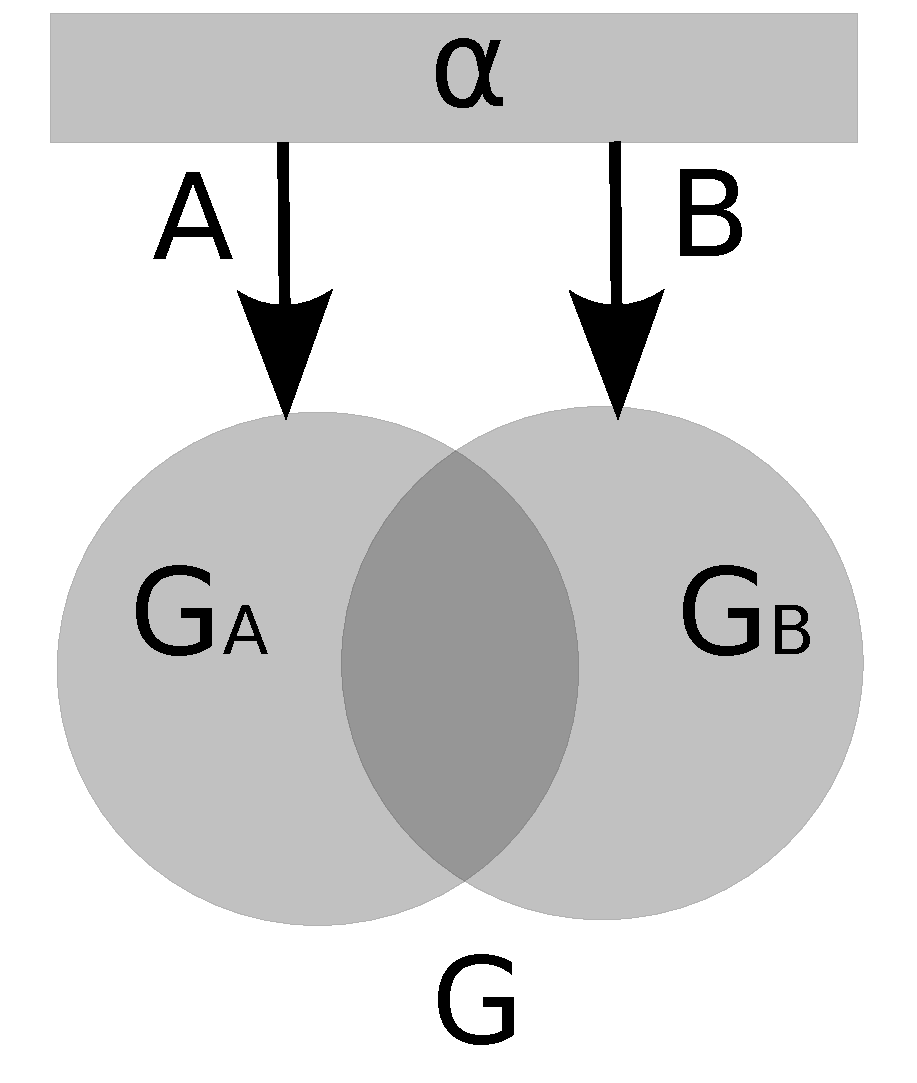
\includegraphics[height=1.18in]{figs/graphmodel2}
  %\label{fig:graph1}}
% %   \hspace{12pt}%
  \caption{Graph model}%
\label{fig:graphmodel2}
\end{minipage}
\begin{minipage}[t]{0.5\linewidth}
%\end{wrapfigure}
%\begin{wrapfigure}{r}{1.0in}
  \centering
% %   %\subfloat[Initially, the owner node $v$ publishes the object]
  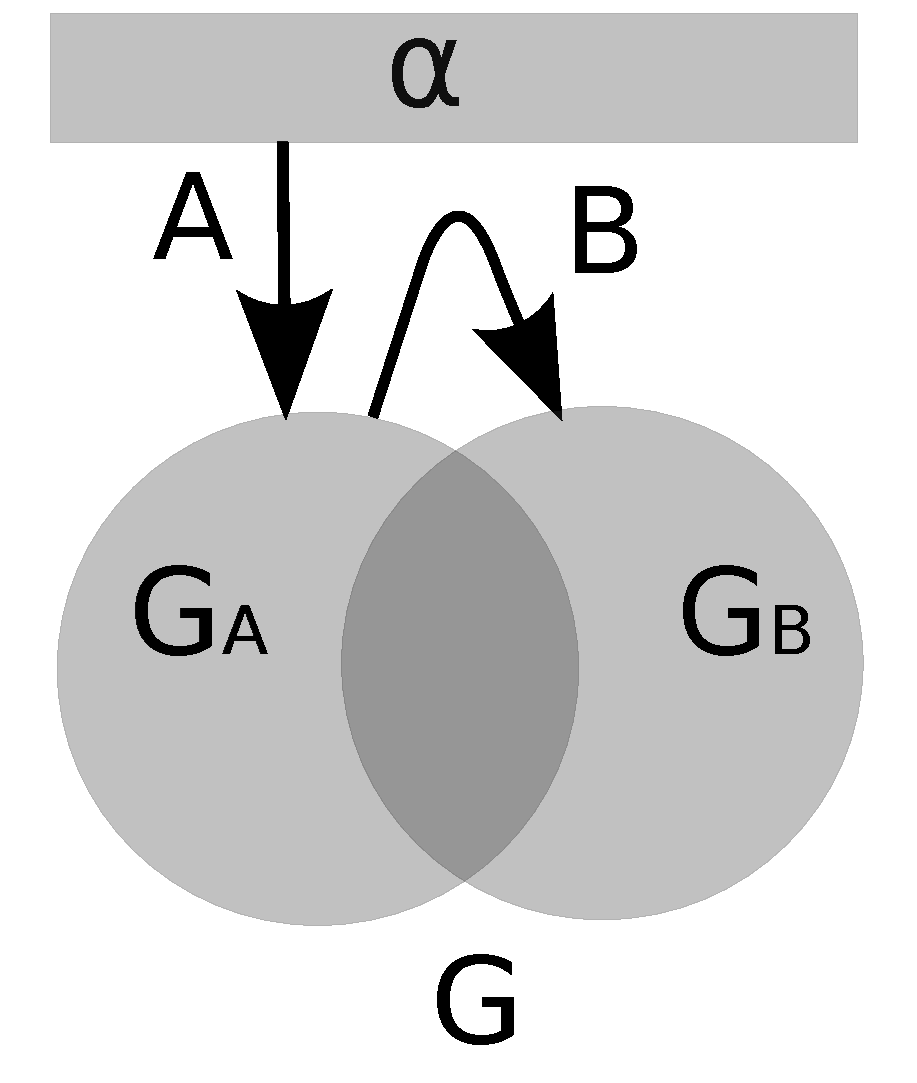
\includegraphics[height=1.18in]{figs/graphmodel2b}
  %\label{fig:graph1}}
% %   \hspace{12pt}%
  \caption{Subgraph model}%
\label{fig:graphmodel3}
\end{minipage}
\end{figure}

Our algorithm uses three phases to perform garbage collection. The three phases are $Phantomize$, $Recover$ and $CleanUp$. The $Phantomization$ phase is a kind of search that marks (i.e. phantomizes) nodes which have lost strong support. The $Recovery$ phase unmarks the nodes, reconnecting the affected subgraph to strong links. If $Recovery$ fails to rebuild links, the $CleanUp$ phase deletes them. The algorithm progresses through all three phases in the order (1. $Phantomize$, 2. $Recover$ and 3. $CleanUp$) and transitions only when there are no more operations left in the current phase. Our algorithm is concurrent because the garbage collection on different subgraphs can proceed independently until, and unless they meet.

If $G$ is the given graph and $\alpha$ is the root set prior to any deletions (see Fig.~\ref{fig:graphmodel2}), $\alpha = \{A, B\}$, and $\alpha = \{ A \}$ after deletions, then
$G$ will become $G_A$, the nodes reachable from $A$.
Thus, $G = G_A \cup G_B$  initially, and
the garbage due to the loss of  $B$ will be $\Gamma_B$.
$$\Gamma_B = G_B - (G_A \cap G_B).$$
During phantomization, all nodes in $\Gamma_B$ and some nodes in $G_A \cap G_B$ will be marked. During recovery, the nodes in $G_A \cap G_B$ will all be unmarked. Hence,
after the $Recovery$ phase, all nodes in $G_A \cap G_B$ will be strongly connected to $A$.
The final phase $CleanUp$ discards the marked memory, $\Gamma_B$.

The above discussion holds equally well if instead of being a root, $B$ is the only strong
link connecting subgraph $G_A$ to subgraph $G_B$. See Fig.~\ref{fig:graphmodel3}.

 %\subsection{Algorithm Design}


% \begin{figure}[h!]
%   \centering
% % %   %\subfloat[Initially, the owner node $v$ publishes the object]
%   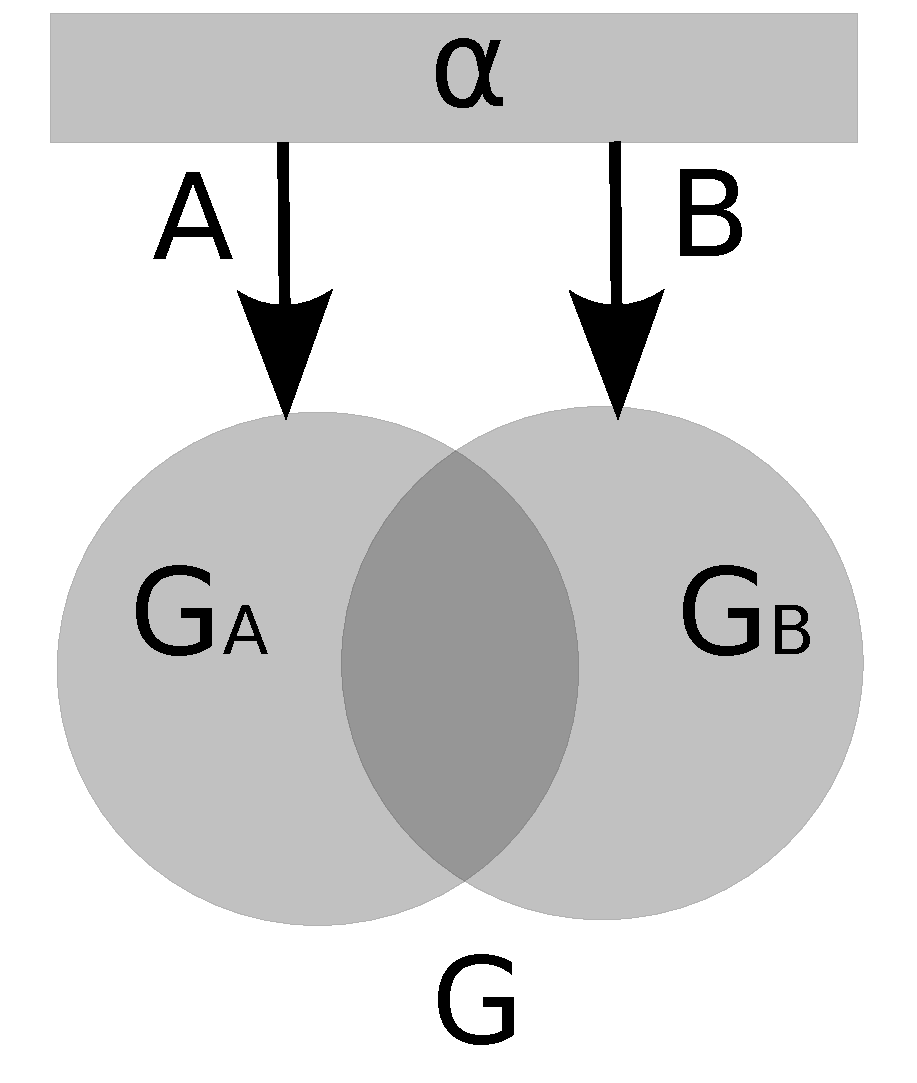
\includegraphics [height=2.5in,width=3.3in] {figs/graphmodel2}
%   %\label{fig:graph1}}
% % %   \hspace{12pt}%
%   \caption{Graph Model}%
%    \label{fig:graphmodel2}
%   \end{figure}







\begin{theorem}[Cycle Invariant]
\label{theorem:cycleinvariant}
No strong cycles are possible, and all cycles formed in the graph should have at least one weak or phantom edge in the cyclic path.
\end{theorem}
\begin{proofs}
This invariant should be maintained through out the graph for any cycles for the algorithm. This property ensures the correctness of the algorithm and the definition of the stable graph. In the rules below, the edge being created is $E$, the source node (if applicable) is called $S$, the target node is $T$. The edge creation rules state: %Assume a graph $G$ that has nodes $a_1$, $a_2$, $a_3$ ... $a_n$. If the edges formed between the nodes create a simple cycle, then by the edge creation rules,
\begin{enumerate}
\setcounter{enumi}{-1}
\item Roots always count as strong edges to nodes.
\item Edge $E$ can be strong if $S$ has no incoming strong edges from other nodes, i.e. if there is no node $C$ with a strong edge to $S$, then $E$ can be created strong. Thus, $S$ is a source of strong edges.
\item A new edge $E$ can be strong if node $T$ has no outgoing non-phantom edges, and $S \neq T$. Thus, $T$ is a terminus of strong edges.
\item A new edge $E$ is strong if $T$ is phantomized and $S$ is not. Thus, $T$ is a terminus of strong edges.
\item A new edge $E$ is weak otherwise. %only if the nodes already have a positive strong count and has outgoing edges, or if it is a self reference.
\item Edge $E$ can only be converted to strong if $T$ is phantomized.
\item A new edge $E$ must be phantom if the node $S$ is phantomized.
\end{enumerate}
Any change described by the above rules regarding strong edges results in one of the nodes becoming a source or terminus of strong edges.
Hence, no strong cycles are possible.
\end{proofs}



%Assume the nodes $a_1$, $a_2$, $a_3$...$a_n$ form a linear chain and the first node $a_1$ is supported the root $A$ in the graph $G$. As we know the nodes are created in the node listed, it was always safe to create each and every edges in the graph to be strong up until now. This makes all nodes in the graph to acquire a positive strong node which signifies the node if they are strongly reachable from any root. When the node $a_n$ creates an edges to $a_1$ to create a cycle, the edge should not be strong. The creation edge rule heuristically says that outgoing edges from the $a_1$ might transitively reach $a_n$ and create a cycle. So it is always safe to create a weak edge in this scenario. So a node with incoming weak edge is not always sign of cycle membership. So in any event, when an edges creates a cycle the edges receiver always has a outgoing edge and a positive strong count. That outgoing edge in the edge receiver should have a path to the node that closing the cycle to form a cycle. So the weak edges in the closing edge of cycle is inevitable by the rules. So thus all cycles formed in graph has at least a weak edge.
%\end{proofs}
%\begin{theorem}[termination]
%Any mutation in the graph $G$ will terminate with $G'$.
%\end{theorem}

%\begin{theorem}[termination]
%Any mutation in the graph $G$ will terminate with $G'$.
%\end{theorem}
%
%\begin{proofs}
%
%
%Assume a graph $G$ is a $Simple Cycle$ and $G$ is supported by roots $A$ and $B$. As $A$ and $B$ both can reach all the nodes in the Graph $G$
%$$G_A \equiv G_B (\because G_A \subseteq G_B)$$
%We prove the termination property by contradiction. If we assume a traversal  is non-terminating, it is only possible if the traversal does not remember the path traversed. This contradicts the marking process which  places the footprints the path traversed. So a graph cannot be traversed indefinitely if there is a mark in the visited node. If there is possibility  that concurrently marks are placed in the  graph $G$ by $A$ and $B$ is replacing the mark as it recovers, then it will indefinitely process the cycle as marking is replace by recovery (unmarking) in the graph. This also contradicts that graph does not do two different phases concurrently. So this show a graph cannot be traversed indefinitely. An action in the one phase can instantiate the action in the same phase or different phase which is eventually marking more nodes in graph or unmarking more nodes but not both at the same time. So the algorithm terminates once the affected nodes are processed. So algorithm always terminates in finite number of steps.
%\end{proofs}

\begin{theorem}[Termination]
\label{theorem:termination}
Any mutations to a stable graph $G$ will take $\cO(N)$ time steps to form a
new stable graph $G'$, where $N$ is number of edges
in the affected subgraph.
\end{theorem}

\begin{proofs}
By {\it stable graph} we mean a graph in which all nodes are strongly connected
from the roots and no phantom links or phantomized nodes are present. Mutations
which enlarge the graph, e.g. adding a root, or edge are constant time
operations since they update the counters and outgoing edge list in a node.
Mutations which diminish the graph, e.g. deleting roots, or edges potentially
begin a process of $Phantomization$, which may spread to any number of nodes in
$G$.
%The Phantomization process terminates if it fails to take away the strong link from a node, if it reaches a node which is already phantomized, or if it reaches a node with no outgoing links. Hence, the Phantomization process cannot take more steps than there are nodes and edges in the affected subgraph graph, and can only traverse a link once.

%Once the Phantomization process begins, the Recovery process begins. The Recovery process traverses each node that lost its last strong link during Phantomization and, if successful, spreads through its outgoing links. It terminates if it reaches an object that already has a strong count greater than zero. Like Phantomization, the process can, at most, spread to all nodes and follow all links in the Phantomized subgraph, and can only traverse a link once.


To prove the algorithm is linear we have to prove that each of the three phases in
the algorithm is linear in time. Without loss of generality, consider the graph
in Fig.~\ref{fig:graphmodel2} (or, equivalently, Fig.~\ref{fig:graphmodel3}). In this graph there are two sets of root links
$A$ and $B$ leading into graph $G$. The graph has three components $G_A$, $G_B$,
$G_A \cap G_B$. So,
$$G_A \cap G_B \subset G_A$$ and
$$G_A \cap G_B \subset G_B,$$
where $\pi_A$ and $\pi_B$ are only reachable  by $A$ and $B$, such that
$$\pi_A = G_A - G_A \cap G_B,$$
$$\pi_B = G_B - G_A \cap G_B.$$
$Phantomization$ starts when a node attempts to convert its weak links to
strong, and marks a path along which strong links are lost. $Phantomization$
stops when no additional nodes in the affected subgraph lose strong
support. In Fig.~\ref{fig:graphmodel2} (or Fig.~\ref{fig:graphmodel3}), the marking process will touch at least
$\pi_B$, and at most, all of $G_B$. The marking step affects both nodes and
edges in $G_B$ and ensures that graph is not traversed twice. Thus, $Phantomization$
will take at most $\cO(N)$ steps to complete where
$N$ is the number of edges in $G_B$.

$Recovery$ traverses all nodes in $G_B$ identified during
$Phantomization$. If the node is marked and has a strong count, it unmarks
the node and rebuilds its outgoing edges, making them strong or weak according to
the rules above. The nodes reached by outgoing links are, in turn,
$Recovered$ as well. Since $Recovery$ involves the unmarking of nodes, it is
attempted for every node and edge identified during phantomization, and can
happen only once, and can take at most $\cO(N)$ steps to complete.

Once the $Recovery$ operations are over, then $CleanUp$ traverses the nodes in
the recovery list. For each node that is still marked as phantomized, the node's
outgoing links are deleted. At the end of this process, all remaining nodes will
have zero references and can be deleted. Because this operation is a single
traversal of the remaining list, it too is manifestly linear.
\end{proofs}

\begin{theorem}[Safety]
Every node collected by our algorithm is indeed garbage and no nodes reachable by roots are collected.
\label{theorem:safety}
\end{theorem}
\begin{proofs}
\begin{comment}
{\color{green}
We say that a garbage collection algorithm is $safe$ if every object collected
is indeed garbage. That is, an object being cleaned up should not be reachable
from any roots.

A node is said to be prematurely deleted if the node is still reachable from some
root. So in order to prove the safety, the algorithm should prove it never
prematurely deletes a node that is reachable at any point in time.

We prove the safety by contradiction. Assume that graph $G$ at time $t$ is
stable. Assume that at time $t' > t$, an edge is removed from the set such that
node $V$ will be prematurely deleted. This means that $V$ must lose all its
strong links. The result must be that it has weak or phantom incoming links, otherwise
it should be deleted. If it has weak or phantom links, however, $V$ will
be phantomized.

If, at the conclusion of the $Phantomization$, $V$ has any non-phantom
references, then at least one will be strong, and $V$ will not collected. This contradicts our
assumption, therefore, $V$ must
only have phantom links at the end of $Phantomization.$

During the $Recovery$ phase, each phantomized node is checked for the presence of
weak or strong links and recovered if it is. If any are present, the phantom links
on $V$ will be rebuilt. Therefore, $V$ must be part of
a set of nodes which only contain phantom links. If this is so, then there can be
no root links connected to any of the objects in the set, and the whole set must
be garbage. This contradicts our assumption that $V$ was prematurely deleted.

Consider now the scenario where just after $Phantomization$ and just before $Recovery$, an edge is removed
from $V$, and just after an attempt to recover $V$ the edge is re-established.
In this case, if the live system attempts to remove a strong edge after $Phantomization$, the
edge is instead transferred to the collector thread allowing the collector thread
to handle the request at a later time. See Algorithm~\ref{algorithm:addtocollector}.
}
\end{comment}
Garbage is defined as a graph not connected to any roots. If the garbage graph contains
no cycles, then it must have at least one node with all zero reference counts. However,
at the point it reached all zero reference counts, the node would have been collected, leaving
a smaller acyclic garbage graph. Because the smaller garbage graph is also acyclic, it must lose
yet another node. So acyclic graphs will be collected.

If a garbage graph contains cycles, it cannot contain strong cycles by
Theorem~\ref{theorem:cycleinvariant}. Thus, there must be a first node in the
chain of strong links. However, at the point where a node lost its last strong
link, it would have either been collected or phantomized, and so it can not
endure. Since there no first link in the chain of strong links can endure, no
chain of strong links can endure in a garbage graph. Likewise, any node having only weak incoming
links will phantomize. Thus, all nodes in a garbage graph containing cycles
must eventually be phantomized.

If such a state is realized, $Recovery$ will occur and fail, and $Cleanup$
will delete the garbage graph.

Alternatively, we show that an object reachable from the roots will not be collected.
Suppose $V^C$ is a node and there is an acyclic chain of nodes
$ Root \rightarrow ... \rightarrow V^A \rightarrow V^B \rightarrow ... \rightarrow V^C$.
Let $V^A$ be a node that is reachable from a root, either directly or by some chain of references.
If one of the nodes in the chain, $V^B$, is connected to $V^A$
and supported only by weak references, then
at the moment $V^B$ lost its last strong link it would have phantomized and converted any
incoming weak link from $V^B$ to strong. If $V^B$ was connected by a phantom link from $V^A$,
then $V^B$ is on the recovery list and will be rebuilt in $Recovery$. This logic can be
repeated for nodes from $V^B$ onwards, and so $V^C$ will eventually be reconnected by
strong links, and will not be deleted.
\label{safety}
\end{proofs}

\begin{theorem}[Liveness]
\label{theorem:liveness}
For a graph of finite size, our algorithm eventually collects all unreachable nodes.
\end{theorem}
\begin{proofs}
We say that a garbage collection algorithm is $live$ if it eventually collects
$all$ unreachable objects, i.e. all unreachable objects are collected and never
left in the memory.
\begin{comment}
Assume that object $V$ becomes garbage but is not collected. If at any time, the
strong, weak, and phantom count on $V$ are all zero, it will be collected.
%Therefore, by the logic used in Theorem~\ref{theorem:safety}, all $V$'s incoming links must become phantomized. If it is phantomized, it
Therefore it has links. However, it must have lost its last strong link, and failed to gain a new one by phantomizing, or it is not garbage.
Therefore, it must be phantomized, and all its incoming edges must be phantoms.
If it is phantomized, it will be tested during $Recovery.$ Since
$V$ is garbage by assumption, recovery must fail. Since it was not
recovered during $Recovery$, it must be part of a set of nodes with
all phantom links. However, it is equally true that if a $Recovery$ is
attempted, a $CleanUp$ will also be attempted and $V$ will be deleted. This
contradicts our assumption that $V$ will not be deleted by our garbage collector after becoming
unreachable in a finite number of steps.
\end{comment}

The only stable state for the graph in our garbage collection is one in which all nodes
are connected by strong links, because any time the last strong link is lost a chain of
events is initiated which either recovers the links or deletes the garbage. Deletion of
a last strong link can result in immediate collection or $Phantomization.$ Once $Phantomization$
begins, it will proceed to completion and be followed $Recovery$ and $Cleanup.$ These
operations will either delete garbage, or rebuild the strong links. See Theorem~\ref{theorem:safety}.
%\end{comment}
\end{proofs}

Note that the live system may create objects faster than the
$Phantomization$ phase can process. In this case, the $Phantomization$ phase will
not terminate.
However, in Theorem \ref{theorem:liveness} when we say the graph be ``of finite size'' we
also count nodes that are unreachable but as yet uncollected,
which enables us to bound the number of nodes that are being added while the $Phantomization$ is in progress.
%, and it is for this
%objection, and similar objections, that we added the qualification that the
%graph be of finite size.
On a practical level, it is possible for garbage to be
created too rapidly to process and the application could terminate with an out-of-memory error.

\section{Experimental Results}
\label{section:experimental}
To verify our work, we modeled the graph problem described by our garbage
collector in Java using fine-grained locks. Our implementation simulates the mutator and collector
behavior that would occur in a production environment. Our mutator threads create, modify, and
delete edges and nodes, and the collector threads react as necessary. This prototype
shows how a real system should behave, and how it scales up with threads.

We also developed various test cases to verify the correctness of the garbage
collector implementation. Our test cases involve a large cycle in which the root
node is constantly moved to the next node in the chain (a ``spinning wheel''), a doubly linked list
with a root node that is constantly shifting, a clique structure, and various
tests involving a sequence of hexagonal cycles connected in a chain.

In Fig.~\ref{fig:scale} we
collected a large number of hexagonal rings in parallel. This
operation should complete in time inversely proportional to the number of threads
in use, as each ring is collected
independently. The expected behavior is observed.

In Fig.~\ref{fig:overhead} we performed the same test, but to a set
of connected rings. The collection threads
merge, but not immediately, so the collection time goes down with the number of
threads used, but not proportionally because the
collection threads only operate in parallel part of the time.

In Fig.~\ref{fig:linearity}, we perform tests to see whether our garbage
collector is linear. We considered a clique, two different hexagonal cycles (one
is interlinked and other separate), a doubly-linked list, and simple cycles, and
measured the collection time per object by varying the size of the graph and
fixing the collector threads to two all times. The results confirmed that our
collector in indeed linear in time.

Our tests are performed on two 2.6 GHz 8-Core Sandy Bridge Xeon Processors (i.e.
on 16 cores) running Redhat Linux 6 64-bit operating system.

\begin{figure}[h!]
  \centering
% %   %\subfloat[Initially, the owner node $v$ publishes the object]
  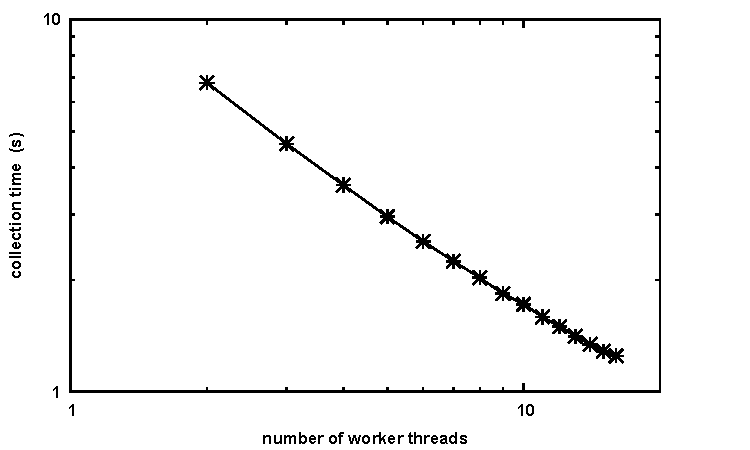
\includegraphics[height=1.8in,width=3.0in]{figs/CleanupTimeperObjectonly16log}
  %\label{fig:graph1}}
% %   \hspace{12pt}%
  \caption{
  A large number of independent rings are collected by various number of
  worker threads. Collection speed drops linearly with the number of
  cores used.
  }
   \label{fig:scale}
  \end{figure}

% % While the algorithm can scale very well with the independent sets, the collector threads working on the shared structure needs synchronization. The testcase that we used for scaling is changed so that all benzene structures are interlinked and collector has to communicate and coordinate their activities based on other collector threads. The algorithm systematically achieves optimized communication and coordination among the multiple collector threads working on the same shared structure. As a result of this, the Fig \ref{fig:overhead} shows the synchronization issues due to multiple threads interacting among each other to cleanup the structure.
\begin{figure}[h!]
  \centering
% %   %\subfloat[Initially, the owner node $v$ publishes the object]
  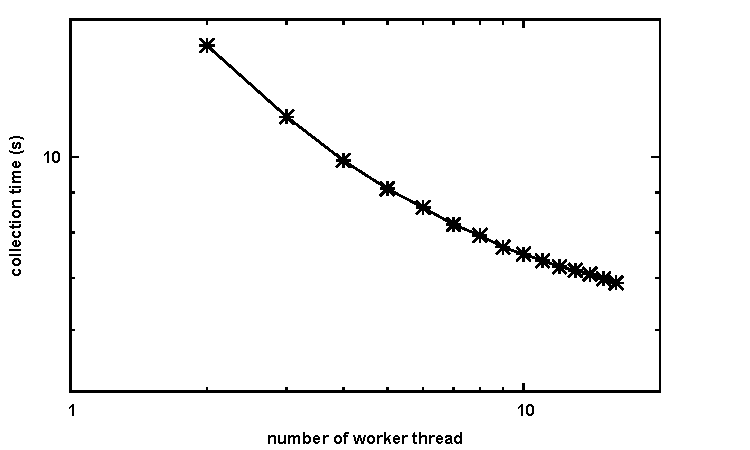
\includegraphics[height=1.8in,width=3.0in]{figs/collapseoverheadonly16log}
  %\label{fig:graph1}}
% %   \hspace{12pt}%
  \caption{A chain of linked cycles is created in memory. The connections are severed,
  then the roots are removed. Multiple collector threads are created and operations
  partially overlap.}
   \label{fig:overhead}
  \end{figure}


\begin{figure}[h!]
  \centering
% %   %\subfloat[Initially, the owner node $v$ publishes the object]
  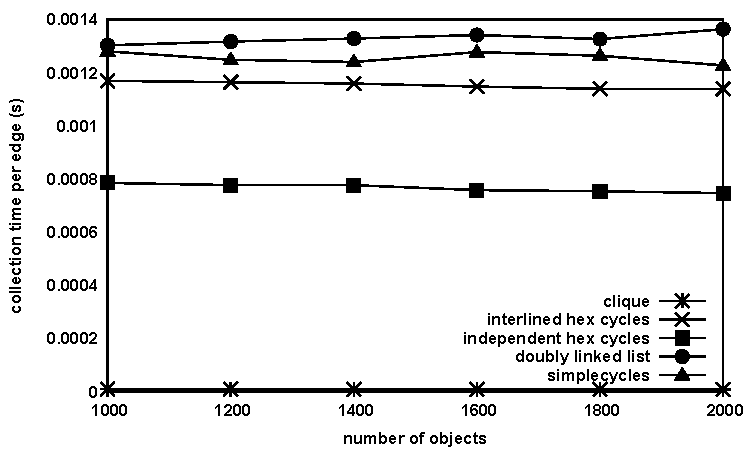
\includegraphics[height=1.8in,width=3.0in]{figs/linearity}
  %\label{fig:graph1}}
% %   \hspace{12pt}%
  \caption{
  Graphs of different types are created at various sizes in memory,
  including cliques, chains of cycles, large cycles, and large doubly
  linked lists. Regardless of the type of object, collection time
  per object remains constant, verifying the linearity of the underlying
  collection mechanism.
  }
   \label{fig:linearity}
  \end{figure}

\section{Future Work}
\label{section:future-work}
There are numerous avenues to explore within this modified Brownbridge framework.

First there are the details of the concurrent operation. While we have explored
the use of merging collector threads upon phantomization, we have not
made use of parallelism within a single collection thread's operations.
Doing so may or may not be desirable, depending on the requirements
for liveness and the compute needs of the application.

Our implementation uses fine-grained locking, but an approach using atomic
variables or atomic transactions should be possible.

Because the situations that lead to nontrivial work are algorithmic, it
should be possible for compilers to optimize instructions to create or
remove links to avoid work. Likewise, it should be possible to build
profiling tools that identify garbage collection
hot spots within a program, and give the programmer the option to take
steps (e.g. re-arrange link structure) to minimize the garbage collector's work.

We also intend to build a high performance distributed version in C++, for
use in High Performance Computing (HPC) systems.
HPC is entering a new phase  in which more complex
simulations are being carried out, covering multiple orders of time and space resolution, and
merging the time evolution of multiple kinds of calculations within a single
calculation. Parallelization of such systems is nontrivial, and increasingly
researchers are moving to dynamic parallelism managed by task queues and
active messages. Numerous frameworks exist,
or are being constructed for this purpose (Charm++~\cite{kale1993charm++},
HPX~\cite{kaiser2009parallex}, Swarm/ETI~\cite{lauderdale2012towards},
UNITAH~\cite{berzins2010uintah}, The Global Arrays
Toolkit~\cite{nieplocha1994global}, etc.)

Until this point, these systems have either required programmers to manage
memory themselves, or use a form of simple reference counting. None of the systems
above offer
an option for global garbage collection capable of reclaiming cycles. Because
garbage collection tends to be a complex, global operation which traces links
throughout memory, it has not been
considered viable in high performance computing to date. However, if the trend
toward increasingly complex multi-scale multi-physics simulations continues, it
may only be a time before garbage collection becomes a requirement.

%The High Performance ParalleX (HPX) effort is
%investigating support for garbage collection in a high performance
%computing context, and the work presented here
%provides a significant milestone in the march toward a future high performance
%implementation. It provides a concurrent implementation where most operations
%are local in nature. Collection operations, even when they contain cycles, are treated
%by operations local to a subgraph and synchronization is only required when
%these subgraphs collide.

%Because the algorithm is intrusive, that
%is because objects need to have knowledge of what pointers they have, it does
%not fit seamlessly with a C++ framework.

%Because of its novel properties, we speculate that this garbage collection
%algorithm might be useful in real time systems. While this effort would not
%be related to our core mission to improve supercomputing, it may nevertheless
%be a worthwhile avenue of study.

%In addition, we hope to discover improvements to the algorithm itself. We hope
%to find a means to minimize or remove the need for a global barrier. At very
%high computer node counts, such barriers may prove to be a significant obstacle.
%We also hope to find a means to make the system fault tolerant, another
%desirable property for computations at large scale.

\section{Conclusion}
\label{section:conclusion}
We have described a garbage collector based on strong and weak reference counts,
proven its validity,
and illustrated its potential advantages over existing systems, including:
\begin{enumerate}
\item It can run at the same time as a live system, using multiple threads if that
is desired, without needing to ``stop the world.''
%It thus may prove useful in soft real-time systems;
\item It has a reduced need to operate on memory compared to collectors because
it only performs nontrivial work when the last strong link is removed;
\item It has a reduced need to trace links in performing its operations, specifically:
\begin{enumerate}
\item When objects do not need to be collected, it is often able to prove this
without completely tracing cycles to which they belong which have support;
\item It remembers stable paths through memory and thus avoids doing work on old objects,
a benefit similar to that derived from generational collectors, e.g. \cite{Printezis:2000};
deletions are occurring;
\item When objects do need to be collected, the collector only needs to trace the cycle twice;
\item The collector operation is local;
\item The collector does not need or use back-pointers;
\end{enumerate}
These advantages should make our collector useful for distributed systems, where traces that
cross node boundaries are likely to be extremely expensive.
\end{enumerate}

Disadvantages include:
\begin{enumerate}
\item An increased memory overhead: three counters and a pointer are required
for each object;
\item An additional cost of pointer creation/mutation;
\item The lack of a fault tolerance protocol;
\item Little effort has, as yet, been devoted to optimization of any implementation. Further reduction of memory and computational overheads may yet be achieved with variations on this algorithm.
%\item The order of deletion in the $CleanUp$ phase is not, at present, guaranteed. This is a potential problem for systems in which finalizers need to run in a certain order, but a system for mitigating this issue is known to us and will be addressed in a future work.
\end{enumerate}

While there are undoubtedly cases for which the increased overheads are unacceptable,
there are just as undoubtedly cases where the potential performance gains make it acceptable.

For distributed applications, a fault tolerance protocol may be of high importance, depending
especially on the reliability of the application components. We expect, however, that variants
of this protocol and synchronization strategies associated with it may be discovered to assist
with these problems.

In short, we feel that collectors based on a system of strong and weak references like
the one we have described here have many potential advantages over existing systems and
should provide a fertile ground for future research and language development.

\section{Appendix}
\subsection{Multi-Threaded Collector}
\label{singlethread}
Note that in the following sections, locks are always obtained in canonical order that avoids deadlocks. Unlock methods unlock the last set of items that were locked.

The lists on the collectors are thread-safe.

The collector object is itself managed by a simple reference count. Code for incrementing and decrementing this count is not explicitly present in the code below.

A reference implementation is also provided ~\cite{url:refimpl}.

\begin{algorithm}[ht]
{\small
\tcp{LinkSet creates a new link,
  and decides the type of the link to create.}
{\bf LinkSet(link,node)}:\\
\quad {lock (link.Source,node)}\\
\quad {\bf if} node == NULL {\bf then}\\
\quad \quad LinkFree(link)\\
\quad \quad link.Target = NULL\\
\quad {\bf EndIf}\\
\quad {\bf if} link.Target == node {\bf then}\\
\quad \quad {\bf Return}\\
\quad {\bf EndIf}\\
\quad oldLink = copy(link) \\
\quad link.Target = node\\
\quad {\bf If} link.Source.Phantomized {\bf then}\\
\quad \quad MergeCollectors(link.Source, link.Target)\\
\quad \quad link.PhantomCount++\\
\quad \quad link.Phantomized = True\\
\quad {\bf ElseIf} link.Source == node {\bf then}\\
\quad \quad link.Which = 1 - node.Which\\
\quad \quad node.Count[link.Which]++\\
\quad {\bf ElseIf} node.Links not initialized {\bf then}\\
\quad \quad node.Count[link.Which]++\\
\quad \quad link.Which = node.Which\\
\quad {\bf Else}\\
\quad \quad link.which = 1 - node.Which\\
\quad \quad node.Count[link.Which]++\\
\quad {\bf EndIf}\\
\quad {\bf If} oldLink != NULL\\
\quad \quad LinkFree(oldLink)\\
\quad  {unlock()}\\
}
\caption{LinkSet}
\label{single:algorithm:linkset}
\end{algorithm}
\setlength{\textfloatsep}{0pt}
\begin{algorithm}[ht]
{\small
\tcp{Freeing a link is usually just the decrement of a reference count, but
if it is the last strong count, this could potentially start a Phantomization process.}
%\begin{multicols}{2}
% \tcp{$R$ and $S$ are objects currently in use.}
{\bf LinkFree(link)}:\\
% \tcp*[f]{Create a pointer from object $R$ to some free object}\\
{\Indp
{lock(link.Source,link.Target)}\\
{\bf If} link.Target == NULL {\bf then}\\
\quad {\bf Return}\\
{\bf EndIf}\\
{\bf If} link.Phantomized {\bf then}\\
\quad DecPhantom(link.Target)\\
{\bf Else}\\
\quad link.Target.Count[link.Which]-\,-\\
\quad {\bf If} link.Target.Count[link.Which] == 0 {\bf And} \\
\quad \quad \quad link.Target.Which == link.Which {\bf then}\\
\quad \quad {\bf If} link.Target.Count[1-link.Target.Which] == 0 {\bf And} \\
\quad \quad \quad \quad link.Target.PhantomCount == 0 {\bf then}\\
\quad \quad \quad Delete(node)\\
\quad \quad \quad link.Target = NULL\\
\quad \quad {\bf Else} \\
\quad \quad \quad {\bf If} link.Target.Collector == NULL {\bf then}\\
\quad \quad \quad \quad link.Target.Collector = new Collector()\\
\quad \quad \quad {\bf EndIf}\\
\quad \quad \quad AddToCollector(link.Target)\\
\quad \quad {\bf EndIf} \\
\quad {\bf EndIf}\\
{\bf EndIf}\\
{unlock()}\\
}
}
\caption{LinkFree}
\label{algorithm:linkfree}
\end{algorithm}
\setlength{\textfloatsep}{0pt}
\begin{algorithm}[ht]
{\small
%\begin{multicols}{2}
% \tcp{$R$ and $S$ are objects currently in use.}
% \tcp*[f]{Create a pointer from object $R$ to some free object}\\
\tcp{Adding an object to the collector puts back the strong
count, effectively transferring the source of the strong link
to the collector. It also adds a phantom count, which helps
prevent the clearing of the Collector field.}
{\bf AddToCollector(node)}:\\
{\Indp
{\bf While} True\\
\quad {lock(node,node.Collector)}\\
\quad {\bf If} node.Collector.Forward != NULL {\bf then}\\
\quad \quad node.Collector = node.Collector.Forward\\
\quad {\bf Else}\\
\quad \quad node.Count[node.Which]++\\
\quad \quad node.PhantomCount++\\
\quad \quad node.Collector.CollectionList.append(node)\\
\quad \quad {\bf Break}\\
\quad {\bf EndIf}\\
\quad {unlock()}\\
{\bf EndWhile}\\
}
}
\caption{AddToCollector}
\label{single:algorithm:addtocollector}
\end{algorithm}
%\end{multicols}
\setlength{\textfloatsep}{0pt}
\begin{algorithm}[ht]
{\small
%\begin{multicols}{2}
\tcp{The collector takes away the strong link it made in
AddToCollector().
}
{\bf PhantomizeNode(node,collector)}:\\
{\Indp
{lock(node)}\\
{\bf While} collector.Forward != NULL\\
\quad collector = collector.Forward\\
{\bf EndWhile}\\
node.Collector = collector\\
node.Count[node.Which]-\,-\\
\quad // Prevent deletion while the\\
\quad // node is managed by the Collector\\
{\bf Let} phantomize = False\\
{\bf If} node.Count[node.Which] $>$ 0 {\bf then}\\
\quad {\bf Return}\\
{\bf Else}\\
\quad {\bf If} node.Count[1-node.Which] $>$ 0 {\bf then}\\
\quad \quad node.Which = 1-node.Which\\
\quad {\bf EndIf}\\
\quad {\bf If} {\bf Not} node.Phantomized {\bf then}\\
\quad \quad node.Phantomized = True\\
\quad \quad node.PhantomizationComplete = False\\
\quad \quad phantomize = True\\
\quad {\bf EndIf}\\

{\bf EndIf}\\
{\bf Let} links = NULL \\
{\bf If} phantomize {\bf then}\\
\quad links = copy(node.Links)\\
{\bf EndIf}\\
{unlock()}\\
{\bf ForEach} outgoing link in links\\
\quad PhantomizeLink(link)\\
{\bf EndFor}\\
lock(node)\\
{node.PhantomizationComplete = True}\\
unlock()\\
}
%\end{multicols}
}
\caption{PhantomizeNode}
\label{algorithm:phantomizenode}
\end{algorithm}
\setlength{\textfloatsep}{0pt}
\begin{algorithm}[ht]
{\small
%\begin{multicols}{2}
\tcp{This method describes the
work to be carried out by a
garbage collection thread. Live
objects pointing to this collector, or
Forward pointers from other collectors
contribute to the RefCount field on
the Collector.}
{\bf Collector.Main()}:\\
{\Indp
{\bf While} True \\
\quad WaitFor(Collector.RefCount == 0 {\bf Or} Work to do)\\
\quad {\bf If} Collector.RefCount == 0 {\bf And} No work to do {\bf then}\\
\quad \quad {\bf Break}\\
\quad {\bf EndIf}\\
\quad {\bf While} Collector.MergedList.size() $>$ 0\\
\quad \quad Let node = Collector.MergedList.pop()\\
\quad \quad Collector.RecoveryList.append(node)\\
\quad {\bf EndWhile}\\
\quad {\bf While} Collector.CollectionList.size() $>$ 0\\
\quad \quad Let node = Collector.CollectionList.pop()\\
\quad \quad PhantomizeNode(node,Collector)\\
\quad \quad Collector.RecoveryList.append(node)\\
\quad {\bf EndWhile}\\
\quad {\bf While} Collector.RecoveryList.size() $>$ 0\\
\quad \quad Let node = Collector.RecoveryList.pop()\\
\quad \quad RecoverNode(node)\\
\quad \quad Collector.CleanList.append(node)\\
\quad {\bf EndWhile}\\
\quad {\bf While} Collector.RebuildList.size() $>$ 0\\
\quad \quad Let node = Collector.RebuildList.pop()\\
\quad \quad RecoverNode(node)\\
\quad {\bf EndWhile}\\
\quad {\bf While} Collector.CleanList.size() $>$ 0\\
\quad \quad Let node = Collector.CleanList.pop()\\
\quad \quad CleanNode(node)\\
\quad {\bf EndWhile}\\
{\bf EndWhile}\\
}
}
\caption{Collector.Main}
\label{algorithm:main}
\end{algorithm}
\setlength{\textfloatsep}{0pt}
\begin{algorithm}[ht]
{\small
%\begin{multicols}{2}
{\bf PhantomizeLink(link)}:\\
{\Indp
 {lock(link.Source,link.Target)}\\
 {\bf If} link.Target == NULL {\bf then}\\
\quad  {unlock()}\\
 \quad {\bf Return}\\
 {\bf EndIf}\\
{\bf If} link.Phantomized {\bf then}\\
\quad  {unlock()}\\
\quad {\bf Return} \\
{\bf EndIf}\\
link.Target.PhantomCount++\\
link.Phantomized = True\\
linkFree(link)\\
MergeCollectors(link.Source, link.Target)\\
 {unlock()}\\
}
}
\caption{PhantomizeLink}
\label{single:algorithm:phantomizelink}
\end{algorithm}
\setlength{\textfloatsep}{0pt}
\begin{algorithm}[ht]
{\small
%\begin{multicols}{2}
\tcp{DecPhantom is responsible for removing any reference to
the collector.}
{\bf DecPhantom(node)}:\\
{\Indp
 {lock(node)}\\
node.PhantomCount- -\\
{\bf If} node.PhantomCount == 0 {\bf then}\\
\quad {\bf If} node.Count[node.Which]== 0 {\bf And}\\
\quad \quad \quad node.Count[1-node.Which] == 0 {\bf then}\\
\quad \quad Delete(node)\\
\quad {\bf Else}\\
\quad \quad node.Collector = NULL\\
\quad {\bf EndIf}\\
{\bf EndIf}\\
 {unlock()}\\
}
}
\caption{DecPhantom}
\label{single:algorithm:decPhantom}
\end{algorithm}
\setlength{\textfloatsep}{0pt}

\begin{algorithm}[ht]
{\small
%\begin{multicols}{2}
{\bf RecoverNode(node)}:\\
{\Indp
 {lock(node)}\\
{\bf Let} links = NULL\\
{\bf If} node.Count[node.Which] $>$ 0 {\bf then}\\
\quad WaitFor(node.PhantomizationComplete == True)\\
\quad node.Phantomized = False\\
\quad links = copy(node.Links)\\
{\bf EndIf}\\
 {unlock()}\\
{\bf ForEach} link in links \\
\quad Rebuild(link)\\
{\bf EndFor}\\
}
}
\caption{RecoverNode}
\label{algorithm:recover}
\end{algorithm}
\setlength{\textfloatsep}{0pt}

\begin{algorithm}[ht]
{\small
%\begin{multicols}{2}
{\bf Rebuild(link)}:\\
{\Indp
 {lock(link.Source,link.Target)}\\
{\bf If} link.Phantomized {\bf then}\\
\quad {\bf If} link.Target == link.Source {\bf then}\\
\quad \quad link.Which = 1- link.Target.Which\\
\quad {\bf ElseIf} link.Target.Phantomized {\bf then} \\
\quad \quad link.Which = link.Target.Which\\
\quad {\bf ElseIf} count(link.Target.Links) == 0 {\bf then}\\
\quad \quad link.Which = link.Target.Which\\
\quad {\bf Else}\\
\quad \quad link.Which = 1-link.Target.Which\\
\quad {\bf EndIf}\\
\quad link.Target.Count[link.Which]++\\
\quad link.Target.PhantomCount- -\\
\quad{\bf If} link.Target.PhantomCount == 0 {\bf then}\\
\quad \quad link.Target.Collector = NULL\\
\quad {\bf EndIf}\\
\quad link.Phantomized = False \\
\quad Add link.Target to Collector.RecoveryList\\
{\bf EndIf}\\
 {unlock()}\\
}
}
\caption{Rebuild}
\label{single:algorithm:rebuild}
\end{algorithm}
\setlength{\textfloatsep}{0pt}

\begin{algorithm}[ht]
{\small
%\begin{multicols}{2}
\tcp{After deleting all the outgoing links, decrement
the phantom count by one (i.e. the reference held by
the collector itself). When the last phantom count
is gone, the object is cleaned up.}
{\bf  CleanNode(node)}:\\
{\Indp
 {lock(node)}\\
{\bf Let} die = False\\
{\bf If} node.Count[node.Which]== 0 {\bf And}\\
\quad \quad node.Count[1-node.Which]== 0 {\bf then}\\
\quad  die = True\\
{\bf EndIf}\\
{unlock()}\\
{\bf If} die {\bf then}\\
\quad {\bf ForEach} link in node\\
\quad \quad LinkFree(link)\\
\quad {\bf EndFor}\\
{\bf EndIf}\\
DecPhantom(node)\\
 }
}
\caption{CleanNode}
\label{algorithm:cleanup}
\end{algorithm}
\setlength{\textfloatsep}{0pt}
\begin{algorithm}[ht]
{\small
{\bf  Delete(node)}:\\
{\Indp
\quad {\bf ForEach} link in node \\
\quad \quad LinkFree(link)\\
\quad {\bf EndFor}\\
\quad freeMem(node)\\

 }
}
\caption{Delete}
\label{algorithm:Delete}
\end{algorithm}
\setlength{\textfloatsep}{0pt}

\begin{algorithm}[ht]
{\small
%\begin{multicols}{2}
\tcp{When two collector threads
realize they are managing a common
subset of objects, one defers to
the other. The arguments, source and
target, are both nodes.}
{\bf MergeCollectors(source,target)}:\\
{\Indp
{\bf Let} s = source.Collector\\
{\bf Let} t = target.Collector\\
{\bf Let} done = False\\
{\bf If} s == NULL {\bf And} t != NULL {\bf then}\\
\quad lock(source)\\
\quad source.Collector = t\\
\quad unlock()\\
\quad {\bf Return}\\
{\bf EndIf}\\
{\bf If} s != NULL {\bf And} t == NULL {\bf then}\\
\quad lock(target)\\
\quad target.Collector = s\\
\quad unlock()\\
\quad {\bf Return}\\
{\bf EndIf}\\
{\bf If} s == NULL {\bf Or} s == NULL {\bf then}\\
\quad {\bf Return}\\
{\bf EndIf}\\
{\bf While Not} done\\
\quad  {lock(s,t,target,source)}\\
\quad {\bf If} s.Forward == t and t.Forward == NULL {\bf then}\\
\quad \quad target.Collector = s\\
\quad \quad source.Collector = s\\
\quad \quad done = True\\
\quad {\bf ElseIf} t.Forward == s and s.Forward == NULL {\bf then}\\
\quad \quad target.Collector = t\\
\quad \quad source.Collector = t\\
\quad \quad done = True\\
\quad {\bf ElseIf} t.Forward != NULL {\bf then}\\
\quad \quad t = t.Forward \\
\quad {\bf ElseIf} s.Forward != NULL {\bf then}\\
\quad \quad s = s.Forward \\
\quad {\bf Else}\\
\quad \quad Transfer s.CollectionList to t.CollectionList \\
\quad \quad Transfer s.MergedList to t.MergedList \\
\quad \quad Transfer s.RecoveryList to t.MergedList \\
\quad \quad Transfer s.RebuildList to t.RebuildList \\
\quad \quad Transfer s.CleanList to t.MergedList \\
\quad \quad target.Collector = t\\
\quad \quad source.Collector = t\\
\quad \quad done = True\\
\quad {\bf EndIf}\\
\quad unlock()\\
{\bf EndWhile} \\
}
}
\caption{MergeCollectors}
\label{algorithm:mergecollectors}
\end{algorithm}

\clearpage

\begin{comment}
\acks
%\subsection{Acknowledgements}
We acknowledge the support
of the following grants: The DoE XPRESS proposal
(DE-SC0008714), and the NSF PXGL (1160602).
We thank Frank L\"{o}ffler and Hartmut Kaiser for
helpful conversations.
%Acknowledgments withheld to facilitate double-blind
%review.


\bibliographystyle{abbrvnat}
\bibliography{paper}
%\clearpage
\appendix

%\subsection{Multi-Threaded Collector}
%\label{multithread}
%\input{algo}
\end{document}
\end{comment}